\documentclass[]{article}
\usepackage{geometry}
\geometry{
a4paper,
total={170mm,257mm},
left=20mm,
top=20mm,
}
\usepackage{booktabs} 
\usepackage{longtable}
\usepackage{appendix}
\usepackage{graphicx}
\usepackage{subcaption}
\usepackage{listings}
\usepackage[justification=centering]{caption}
\usepackage{hyperref}
\usepackage{enumitem}
\usepackage[utf8]{inputenc}
\usepackage{float}
\DeclareTextFontCommand{\helvetica}{\fontfamily{phv}\selectfont}
\setlength{\parindent}{4em}
\setlength{\parskip}{1em}
\linespread{1.5}

\usepackage[table]{xcolor}
\usepackage{graphicx}
\usepackage{adjustbox}

\title{PAC2 Desenvolupament del treball - Fase 1}
\date{15 d'Abril 2019}
\author{Vasyl Druchkiv \\ Estudiant del Màster de Bioestadística i Bioinformàtica}
\renewcommand{\contentsname}{Índice}
\usepackage{setspace}


\renewcommand\paragraph{\@startsection{paragraph}{4}{\z@}%
{-2.5ex\@plus -1ex \@minus -.25ex}%
{1.25ex \@plus .25ex}%
{\normalfont\normalsize\bfseries}}

\begin{document}
\maketitle
\makeatletter

\makeatother
\begin{spacing}{0.1}
\tableofcontents
\end{spacing}

\begin{center}
\noindent\rule{8cm}{0.4pt}
\end{center}

\section{Descripció de l'avenç del projecte} 

A data d'avui he desenvolpupat l'aplicació d'anàlisis de les rutes. L'aplicació és completament funcional localment i ofereix l'anàlisi a partir de les bases de dades GO, KEGG i Reactome. A l'apartat \textbf{Input data} l'usuari primer ha d'indicar l'espècie per a totes tres bases de dades. Per les bases de dades de Reactome l'usuari pot elegir entre Homo Sapiens, Rat, Mouse, Celegans, Yeast, Zebrafish, Fly. Per a l’anàlisi GO, a més de les anteriors, hi ha disponibles aquestes espècies addicionals: Arabidopsis, Bovine, Chicken, Canine, Pig, Rhesus, E coli strain K12, Xenopus, Anopheles, Chimp, Malaria, E coli strain Sakai. Hi ha més espècies disponibles per a l'anàlisis KEGG, perquè la funció de \helvetica{culsterProfiler} \helvetica{enrichKEGG()} descarrega les últimes anotacions directament de la base de dades KEGG. Es poden trobar totes les espècies \href{http://www.genome.jp/kegg/catalog/org_list.html}{aquí}. També l'usuari pot buscar l'espècie introduint els termes de cerca. Finalment l'usuari puja l'arxiu amb els gens i els LogRatios provinents de l'estudi de microarrays o NGS. 


\begin{figure}[H]
\caption{Pàgina d'entrada}
\centering
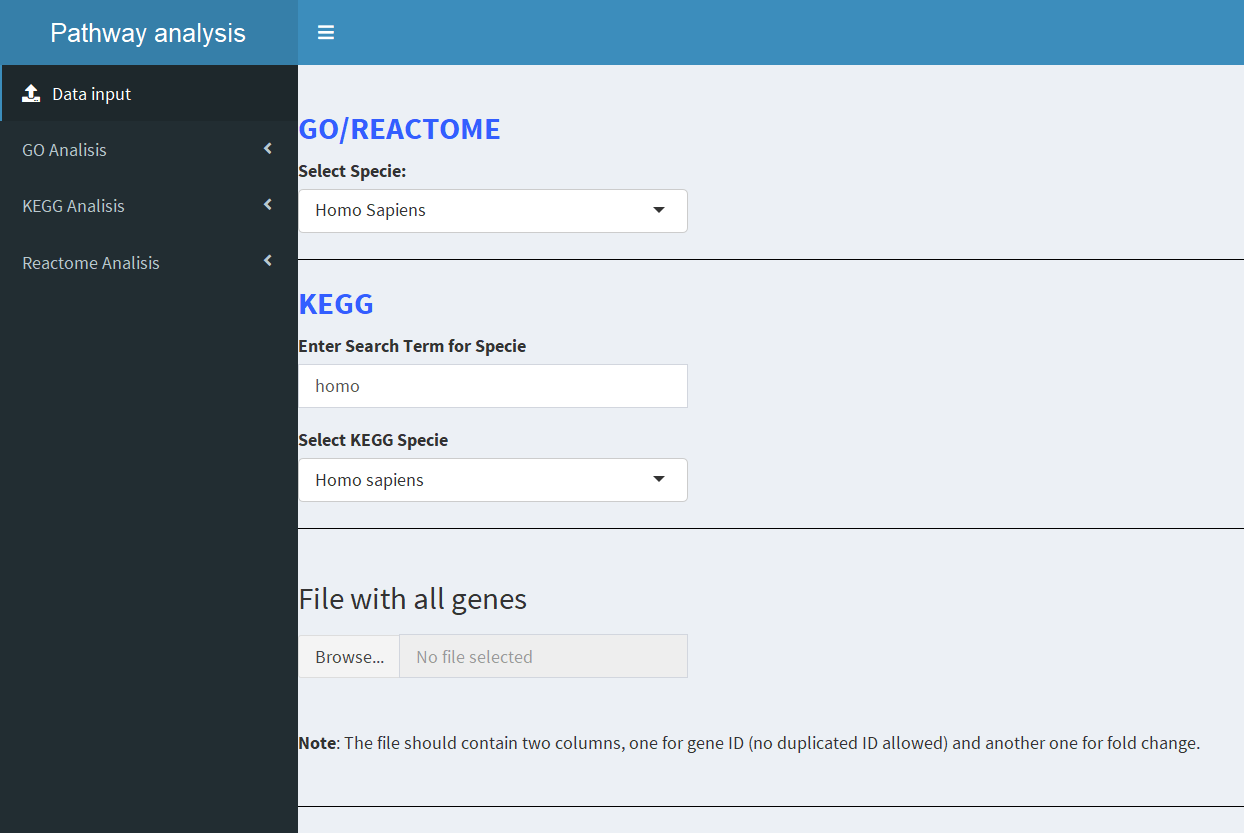
\includegraphics[width=0.9\textwidth]{App_F1}
\end{figure}

L'usuari té la possibilitat d'introduir l'arxiu amb tots els gens i els gens seleccionats. Un cop introduïdes les dades es mostra un petit resum del contingut dels arxius.

\begin{figure}[H]
\caption{El resum de les dades selecció del \textit{cut off} per a l'anàlisi ORA}
\centering
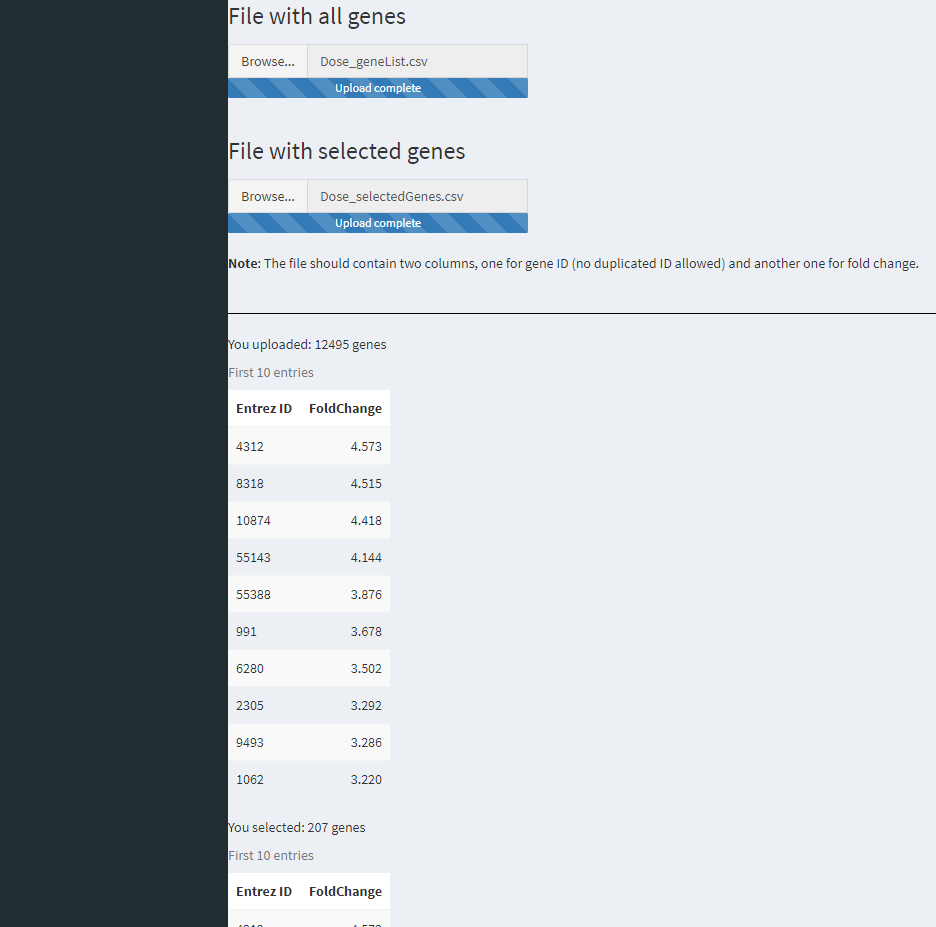
\includegraphics[width=0.9\textwidth]{App_F1b}
\end{figure}


L'aplicació està dividida doncs en 4 parts substancials:

\begin{enumerate}
\item Entrada de les dades;
\item Anàlisi GO;
\item Anàlisi KEGG;
\item Anàlisi Reactome.
\end{enumerate}


L'aplicació ofereix dos mètodes d'anàlisi: d'una banda es pot fer ORA (Over-Representation Analysis) i d'altra banda l'anàlisi GSEA (Gene Set Enrichment Analisis). Recordem que l'ORA consisteix a seleccionar els gens diferencialment expressats i basant-se en GO, KEGG o Reactome comprovar si una de les agrupacions de gens suggerides per aquestes bases de dades està sobre o sotraexpressada en els gens seleccionats. Per dur a terme l'ORA l'usuari té l’opció de definir un \textit{cut-off} de Log-Ratio per formar el conjunt dels gens que s'hi utilitzarà (\textit{gene set}). ORA és una bona eina per veure els efectes grans però els efectes petits se li escapen. Els efectes petits derivats dels gens individuals poden acumular-se en un efecte conjunt substancial el qual ORA no serà capaç de detectar. És aquí on GSEA mostra la seva utilitat. 

Els apartats d'anàlisi (GO, KEGG i Reactome) ofereixen tan representacions comunes com representacions específiques. 

Els anàlisis i representacions \hyperref[sec:ACom]{\underline{en comú}} són:

\begin{itemize}
\item Taula dels resultats ORA;
\item Taula dels resultats GSEA;
\item Gràfic de barres del resultat ORA;
\item Gràfic de punts del resultat ORA;
\item El mapa d'enriquement (Enrichment Map);
\item La xarxa dels gens en categories (Category-gene-network);
\item El gràfic de GSEA.
\end{itemize} 

Les anàlisis \hyperref[sec:ASpec]{\underline{específics}} són:

\begin{itemize}
\item GO $\rightarrow$ Gràfic GO 
\item KEGG $\rightarrow$ Rutes de la base de dades KEGG
\item Reactome $\rightarrow$ Rutes de la base de dades Reactome
\end{itemize}

\begin{figure}[h!]
\centering
\begin{tabular}{ccc}
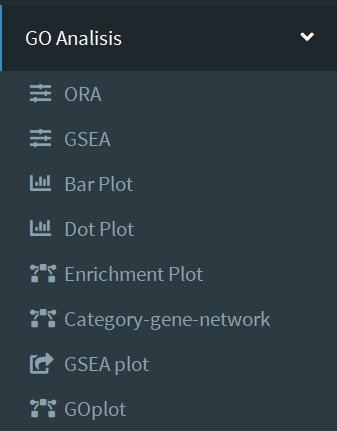
\includegraphics[width=45mm]{App_F2_Items_GO.png} & 
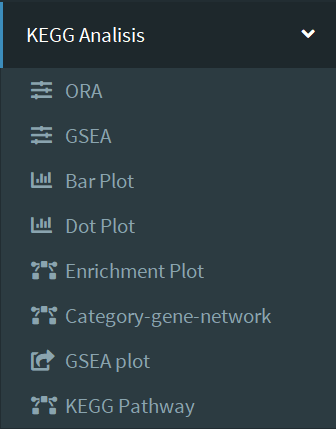
\includegraphics[width=45mm]{App_F3_Items_KEGG.png} &
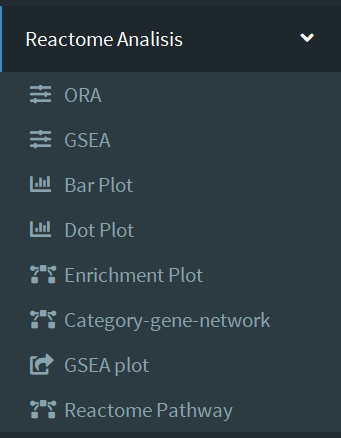
\includegraphics[width=45mm]{App_F4_Items_RA.png} \\
(a) GO & (b) KEGG & (c) Reactome \\
\end{tabular}
\caption{Els elements de les seccions d'anàlisi}
\end{figure}


\begin{table}[H]
\begin{adjustbox}{width=1\textwidth}
\small
\begin{tabular}{|| c | c | l | c | c ||} 
\hline
Base de dades & Mètode & Paquet Bioconductor & Funció & Observació \\ [0.5ex] 
\hline\hline
GO & ORA & clusterProfiler & enrichGO() & Només 7 espècies disponibles \\ 
\hline
GO & GSEA & clusterProfiler & gseGO() & Permutació de gens \\
\hline
GO & Bar-Plot & enrichplot & barplot() & Necessita l'objecte del class enrichResult \\
\hline
GO & Enrichment Map & enrichplot & emapplot() & Necessita l'objecte del class enrichResult \\
\hline
GO & Gene-Concept Network & enrichplot & cnetplot() & Necessita l'objecte del class enrichResult \\
\hline
GO & GO directed acyclic graph & enrichplot & goplot() & Necessita l'objecte del class enrichResult \\
\hline\hline
KEGG & ORA & clusterProfiler & enrichKEGG() & Totes les espècies de KEGG \\ 
\hline
KEGG & GSEA & clusterProfiler & gseKEGG() & Permutació de gens \\
\hline
KEGG & Bar-Plot & enrichplot & barplot() & Necessita l'objecte del class enrichResult \\
\hline
KEGG & Enrichment Map & enrichplot & emapplot() & Necessita l'objecte del class enrichResult \\
\hline
KEGG & Gene-Concept Network & enrichplot & cnetplot() & Necessita l'objecte del class enrichResult \\
\hline
KEGG & Pathway & pathview & pathview() & Cal modificar la funció per guardar els gràfics en el directori temporal \\
\hline\hline
Reactome & ORA & ReactomePA & enrichPathway() & Totes les espècies de KEGG \\ 
\hline
Reactome & GSEA & ReactomePA & gsePathway() & Permutació de gens \\
\hline
Reactome & Bar-Plot & enrichplot & barplot() & Necessita l'objecte del class enrichResult \\
\hline
Reactome & Enrichment Map & enrichplot & emapplot() & Necessita l'objecte del class enrichResult \\
\hline
Reactome & Gene-Concept Network & enrichplot & cnetplot() & Necessita l'objecte del class enrichResult \\
\hline
Reactome & Pathway & ReactomePA & viewPathway() &  \\
\hline
\hline
\end{tabular}
\end{adjustbox}
\caption{Resum de les anàlisis disponibles i recursos de Bioconductor R} 
\end{table}

El llistat de tots els paquets i funcions utilitzats en l’aplicació es troba a \hyperref[sec:A1]{apèndix A}.




\section{Grau de compliment dels objectius}

Recordem el calendari definit al pla de treball.

\begin{figure}[H]
\centering
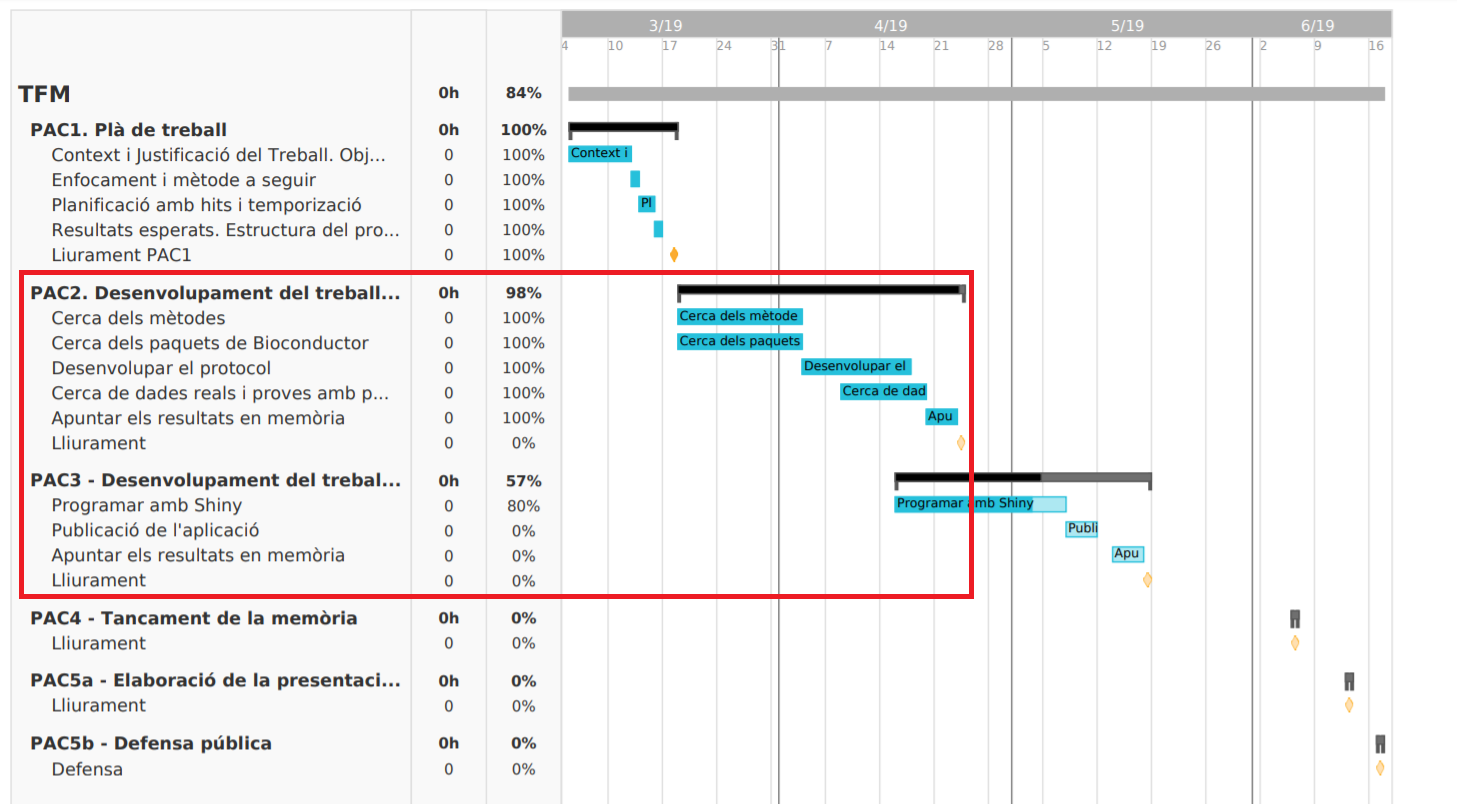
\includegraphics[width=0.9\textwidth]{Calender.png} 
\caption{Diagrama de Gantt}
\end{figure}

Les tasques per a aquesta PAC eren:

\begin{enumerate}
\item \textbf{Cerca dels mètodes}

Els mètodes interessants per a dur a terme l'anàlisi de les rutes són:

\begin{itemize}
\item ORA \cite{boyle2004go}
\item Mètodes GSA
\begin{itemize} 
\item Permutació de les mostres: GSEA \cite{subramanian2005gene}, SAFE\cite{dinu2007improving} com els més representatius;
\item Permutació dels gens: PAGE \cite{kim2005page}, T-Profiler\cite{newton2007random} com els més representatius.
\end{itemize}
\item GAGE (Generally Applicable Gene set Enrichment for pathway analysis) \cite{luo2009gage}
\end{itemize}

Per fer l'aplicació més estructurada i menys complicada he elegit al final els dos mètodes: ORA \cite{boyle2004go} i GSEA \cite{subramanian2005gene}. L'anàlisi GAGE seria un bon \textit{Add-on} però per falta de temps per completar el TFM al final he decidit deixar-ho. 

\item \textbf{Cerca dels paquets de Bioconductor}

El paquet \helvetica{clusterProfiler} de Bioconductor integra els mètodes per dur a terme l'anàlisi de les rutes basant-se en les bases de dades GO, KEGG i Reactome. Els dos mètodes principals són ORA (Overrepresentation analysis) i GSEA (Gene set enrichment Analysis). També inclou les possibilitats de visualització dels resultats suficients per considerar l'anàlisi de les rutes complet. Notem però que el test de permutació a l'anàlisi GSEA implementat per clusterPrifiler es basa en la permutació dels gens i no de les mostres com originalment és proposat per \cite{subramanian2005gene}.

\item \textbf{Desenvolupar el protocol}

Crec que l'aplicació és molt intuitiva i deixa entreveure l'esquema següent:

\begin{figure}[H]
\centering
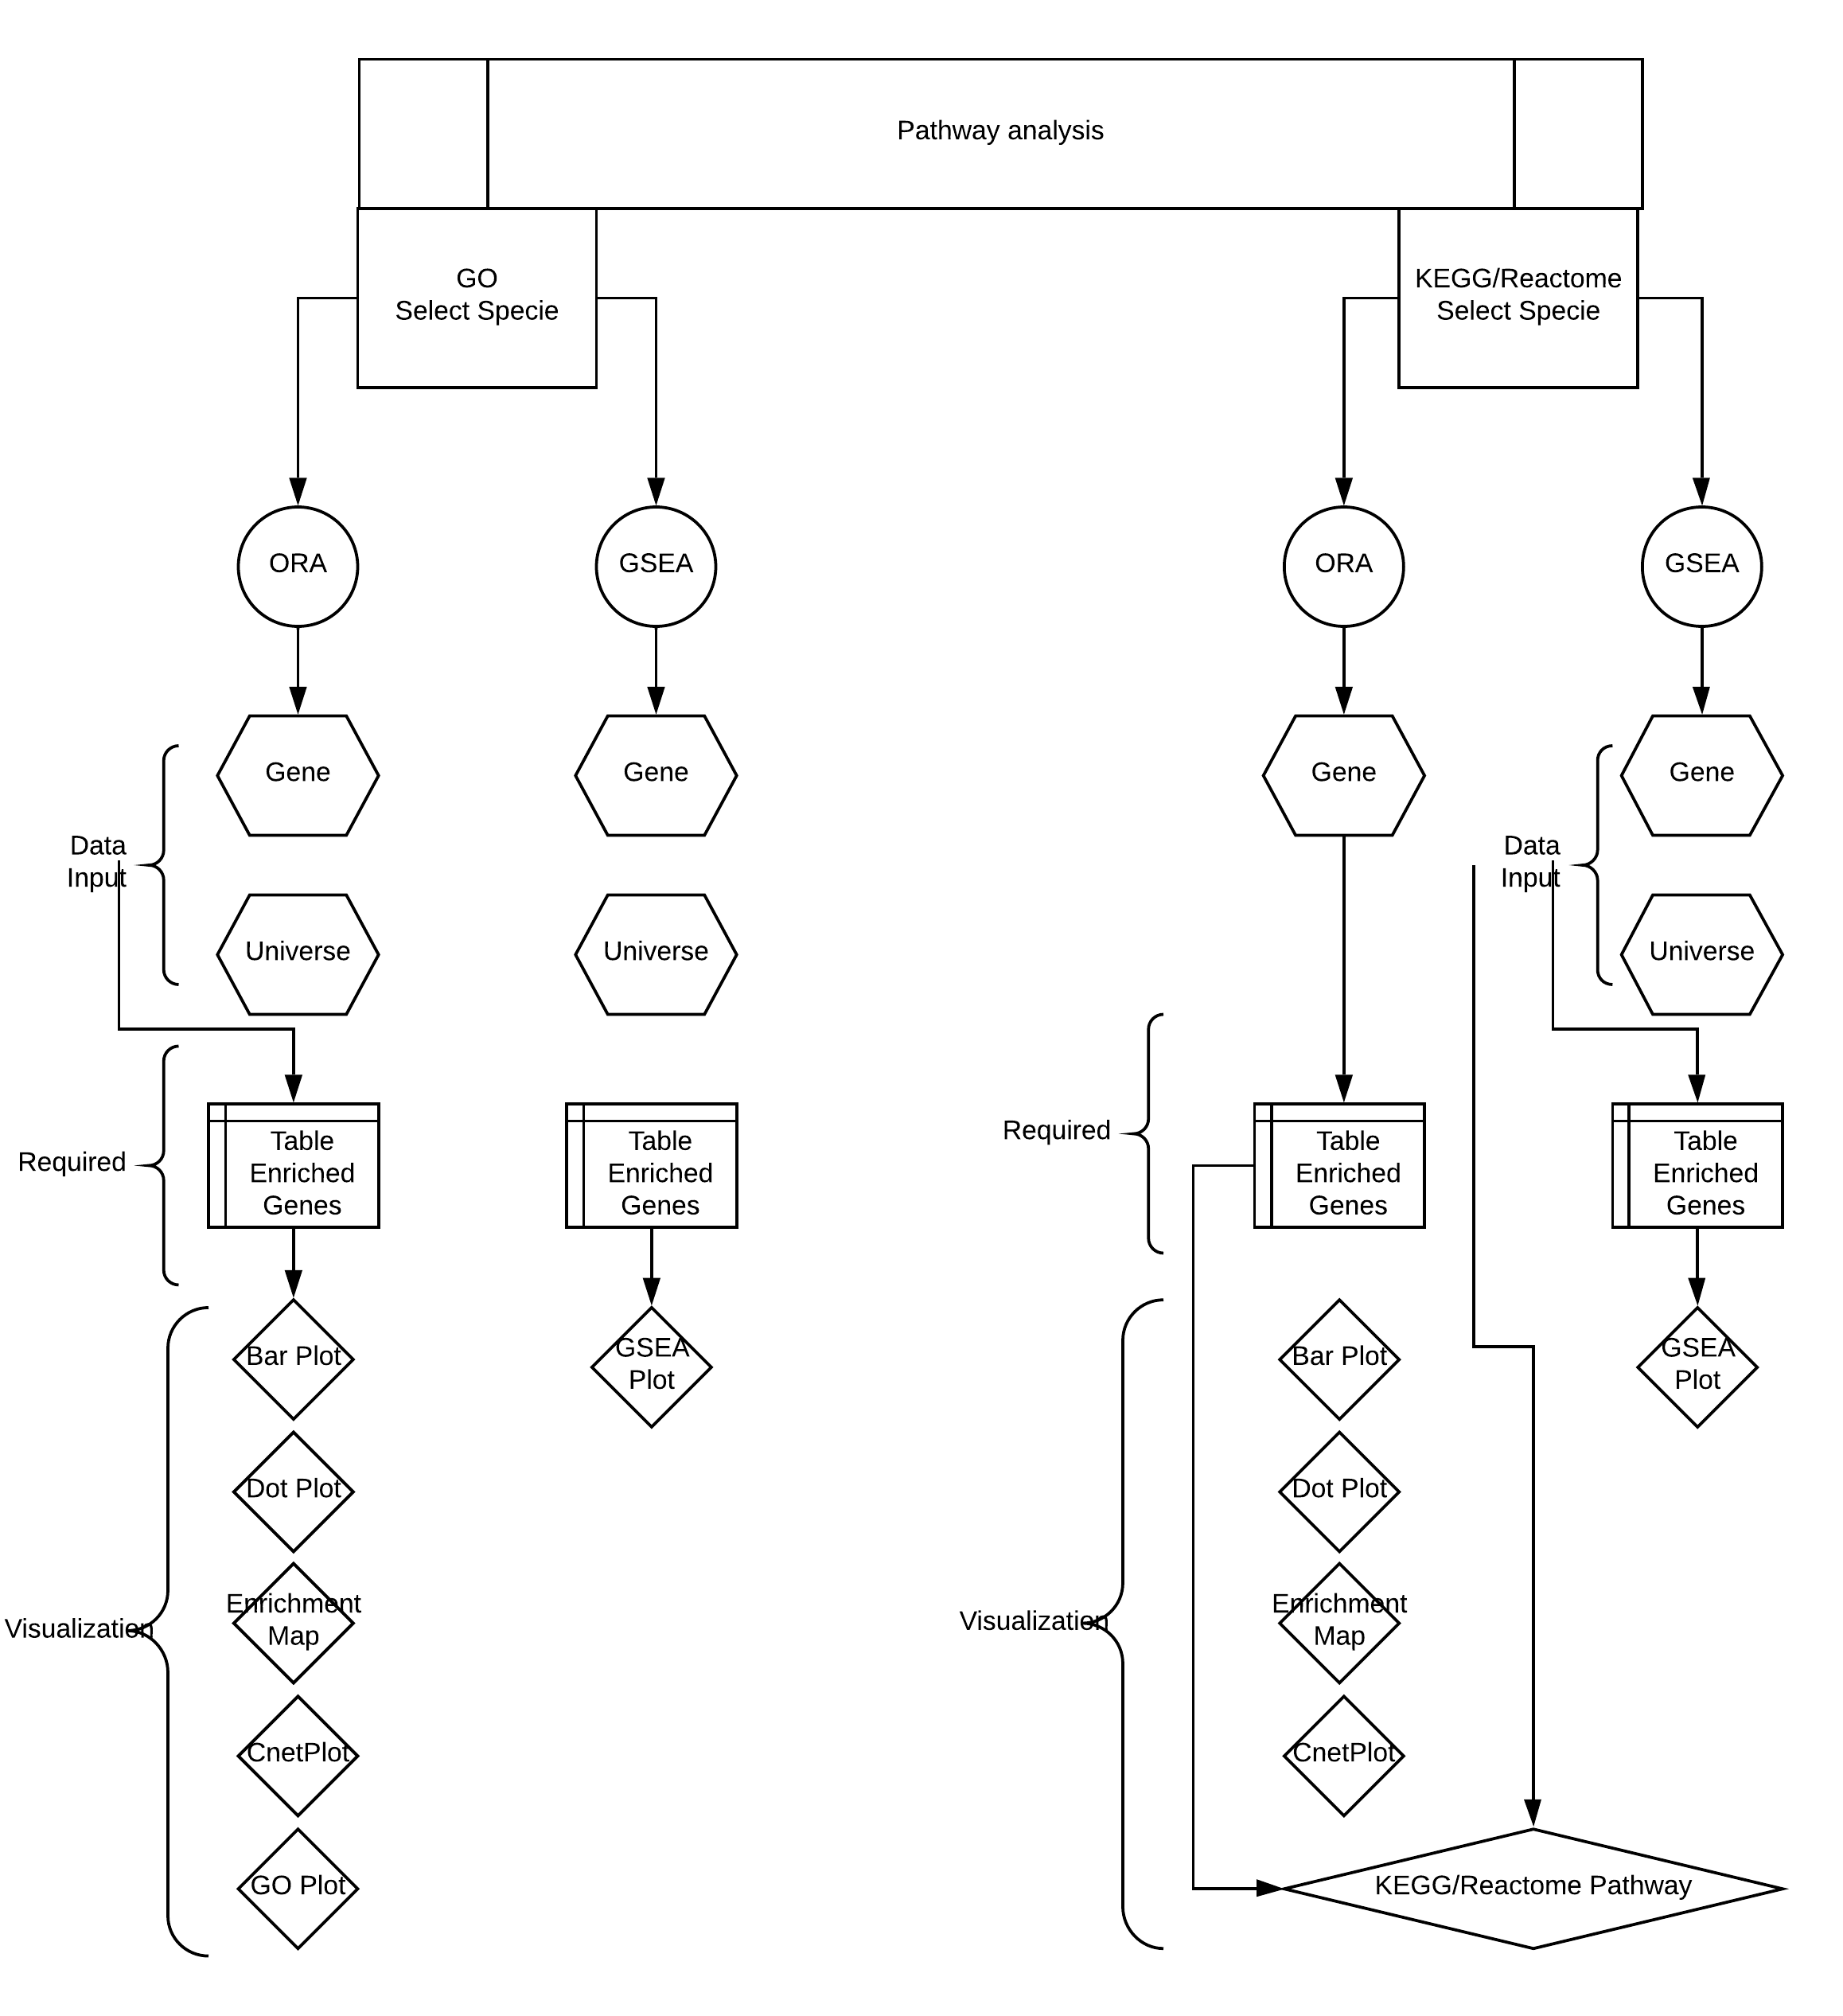
\includegraphics[width=0.9\textwidth]{LucidChart.png} 
\caption{Lucidchart per a l'aplicació}
\end{figure}

D'aquí podem definir per exemple el protocol:
\begin{enumerate}
\item Decidir quin anàlisi vol fer: GO, KEGG o Reactome
\item Seleccionar l'espècie de referència
\item Decidir quin mètode vol implementar: ORA o GSEA i respectivament pujar les dades necessàries.

$\rightarrow$ Per a anàlisi GO tots dos arxius són necessaris: Gens Seleccionats (Gene) i Tots els gens (Universe). 

$\rightarrow$ Per a l'anàlisi KEGG o Reactome les dades necessàries varien: Pel mètode ORA l'arxiu amb els gens seleccionats és suficient. Dos arxius són necessaris pel mètode GSEA.
\item En el cas que volguem fer l'anàlisis ORA seleccionar a l'apartat corresponent (GO, KEGG o Reactome) la pestanya ORA i definir els criteris.

$\rightarrow$ Els gràfics: Bar Plot, Dot Plot Enrichment Map, Cnet Plot, GO Plot (en cas d'anàlisi GO) i els gràfics de les rutes (KEGG/Reactome) es calculen automàticament

\item En el cas que volguem fer l'anàlisi GSEA seleccionar a l'apartat corresponent (GO, KEGG o Reactome) la pestanya GSEA i definir els criteris.

$\rightarrow$ El gràfic GSEA es genera automàticament. Es pot elegir la ruta mitjançant un menú desplegable.

\end{enumerate}

\item \textbf{Cerca de dades i proves amb el protocol}

Aquesta tasca ha resultat ser més difícil. Estic però satisfet que amb l’ajuda del professor he pogut trobar les dades i amb algunes d'elles ja fer les proves. Els detalls els explico en l'apartat \hyperref[sec:ValRes]{Validació dels resultats}.

\item \textbf{Programar amb shiny}

Estic satisfet amb el grau del complement amb aquesta tasca. L'aplicació és ja funcional. D'altra banda noto que ara hi ha molt de codi repetitiu. Encara no he trobat la possibilitat de simplificar-lo. Estic buscant però les solucions.
\end{enumerate}

\section{L'anàlisi comuna de GO, KEGG i Reactome}
\label{sec:ACom}

\subsection{ORA}

\subsubsection{GO}

Per realitzar l'anàlisi ORA per a termes GO s'utilitza la funció \helvetica{enrichGO} del paquet \helvetica{clusterPrifiler}.
\begin{lstlisting}[language=R]
enrichGO(gene, OrgDb, keyType = "ENTREZID", ont = "MF", pvalueCutoff = 0.05, 
pAdjustMethod = "BH", universe, qvalueCutoff = 0.2, minGSSize = 10, maxGSSize = 500, 
readable = FALSE, pool = FALSE)
\end{lstlisting}

He implementat els valors per defecte amb la possibilitat per a l’usuari d'elegir entre:

\begin{itemize}
\item \underline{Ontologies GO} 
\begin{itemize}
\item Molecular function, Biological proces, Cellular Components;
\end{itemize}
\item \underline{Nivell de significació basant-se en els valors de P ajustats}
\begin{itemize}
\item 0.1, 0.05, 0.01, 0.001;
\end{itemize}
\item \underline{Mètode d'ajustament}
\begin{itemize}
\item Holm; Hochberg; Hommel; Bonferroni; BH; BY; FDR; None.
\end{itemize}
\end{itemize}

\begin{figure}[h!]
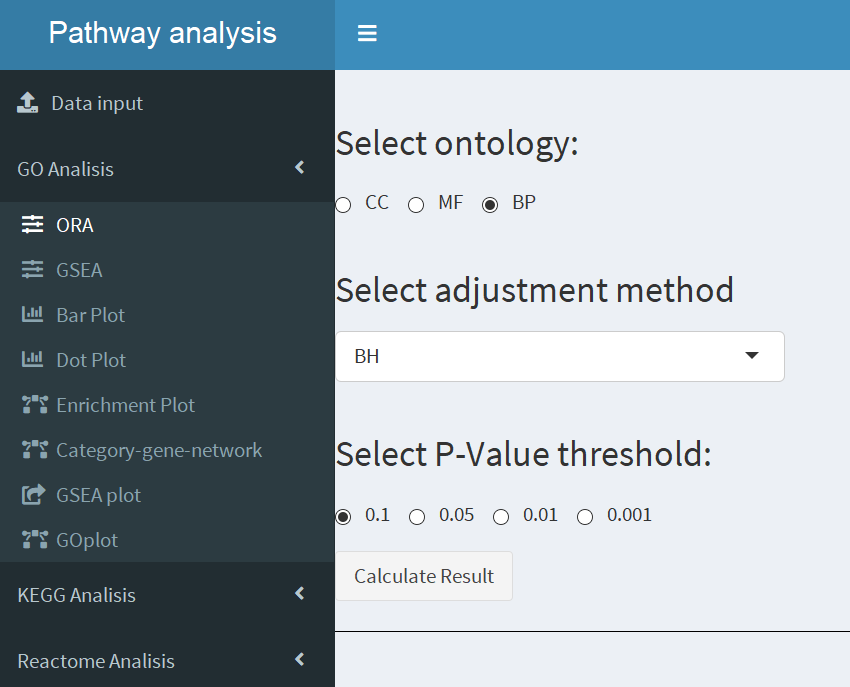
\includegraphics[width=0.9\textwidth]{App_F5_Items_GO_ORA.png}
\caption{Especificació d'ORA dels termes GO}
\end{figure}
L'execució de la funció és un procès temporalment costós. Per aquest motiu he afegit el botó d'acció, en lloc de deixar la funció reactiva. D'aquesta manera l'usuari ha de fer una decisió conscient de repetir l'anàlisi amb altres valors.

Prement el botó apareix la taula i el botó nou mitjançant el qual l'usuari pot descarregar els resultats en format .csv. He formatejat la taula amb els paquets \helvetica{knitr}, \helvetica{kableExtra}, \helvetica{formattable} i \helvetica{dplyr}. Amb els dos últims he afegit les barres de color pel nombre dels gens diferencialment expressats del terme específic de GO i la gradació de color del verd fins al vermell pels valors dels més petits fins els més grans. 

\begin{figure}[h!]
\centering
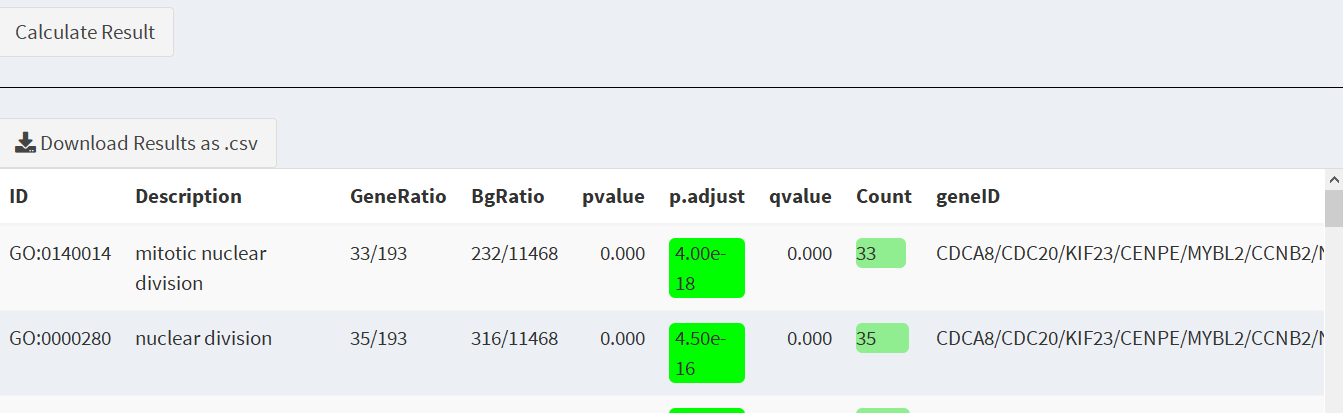
\includegraphics[width=0.9\textwidth]{App_F6_Items_GO_ORA_Table.png} 
\caption{El resultat d'anàlisi ORA. GO.}
\end{figure}

Els camps més interessants de la taula són:

\begin{itemize}
\item \underline{Description}. El nom del terme GO;
\item \underline{GeneRatio}. El quocient: $\displaystyle\frac{\mbox{Nombre dels gens diferencialment expressats que pertanyen al conjunt de gens}}{\mbox{Nombre total dels gens diferencialment expressats}}=\frac{M}{N}$; 
\item \underline{BgRatio}. El quocient: $\displaystyle\frac{\mbox{Nombre dels gens del conjunt d'interès en tota la mostra}}{\mbox{Nombre total dels gens en la mostra}}=\frac{k}{n}$;
\item \underline{pvalue}. Valor de p basat en la distribució hipergeomètrica: $p = 1 - \displaystyle\sum_{i = 0}^{k-1}\frac{{M \choose i}{{N-M} \choose {n-i}}} {{N \choose n}}$
\item \underline{p.adjust}. El valor de P ajustat.
\end{itemize}

\subsubsection{KEGG}

Per l'ORA de base de dades KEGG he utilitzat la funció \helvetica{enrichKEGG()} del paquet \helvetica{clusterProfiler}. 

\begin{lstlisting}[language=R]
enrichKEGG(gene, organism = "hsa", keyType = "kegg", pvalueCutoff = 0.05, 
pAdjustMethod = "BH", universe, minGSSize = 10, maxGSSize = 500, 
qvalueCutoff = 0.2, use_internal_data = FALSE)
\end{lstlisting}



\begin{figure}[H]
\centering
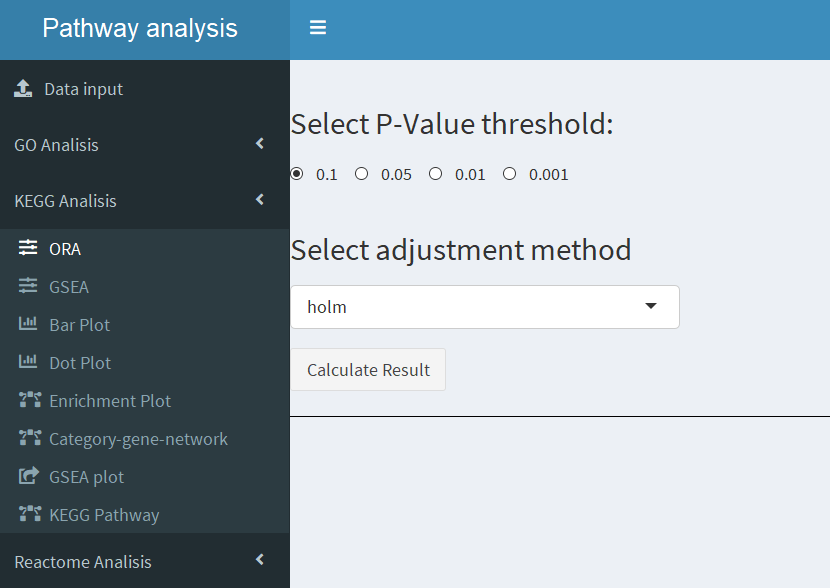
\includegraphics[width=0.9\textwidth]{App_F7_Items_KEGG_ORA.png} 
\caption{Configuració d'anàlisi KEGG}
\end{figure}



Una vegada introduïts els paràmetres i premut el botó \textbf{Calculate} apareix el botó \textbf{Download .csv} i la taula previsualitzada. Els camps de la taula són els mateixos com en l'anàlisi dels termes GO.
\begin{figure}[H]
\centering
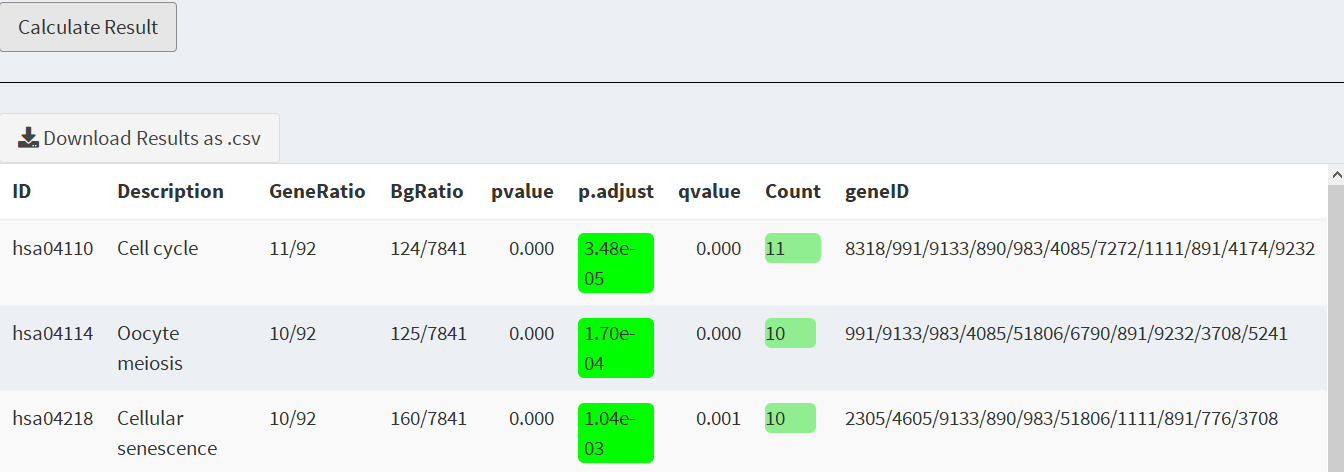
\includegraphics[width=0.9\textwidth]{App_F9_Items_KEGG_ORA_Table.png} 
\caption{El resultat de l'anàlisi ORA. KEGG.}
\end{figure}

\subsubsection{Reactome}
En el cas de Reactome el procediment és similar. La funció usada és \helvetica{enrichPathway()} del paquet \helvetica{ReactomePA}:

\begin{lstlisting}[language=R]
enrichPathway(gene, organism = "human", pvalueCutoff = 0.05,
pAdjustMethod = "BH", qvalueCutoff = 0.2, universe, minGSSize = 10,
maxGSSize = 500, readable = FALSE)
\end{lstlisting}


\begin{figure}[H]
\centering
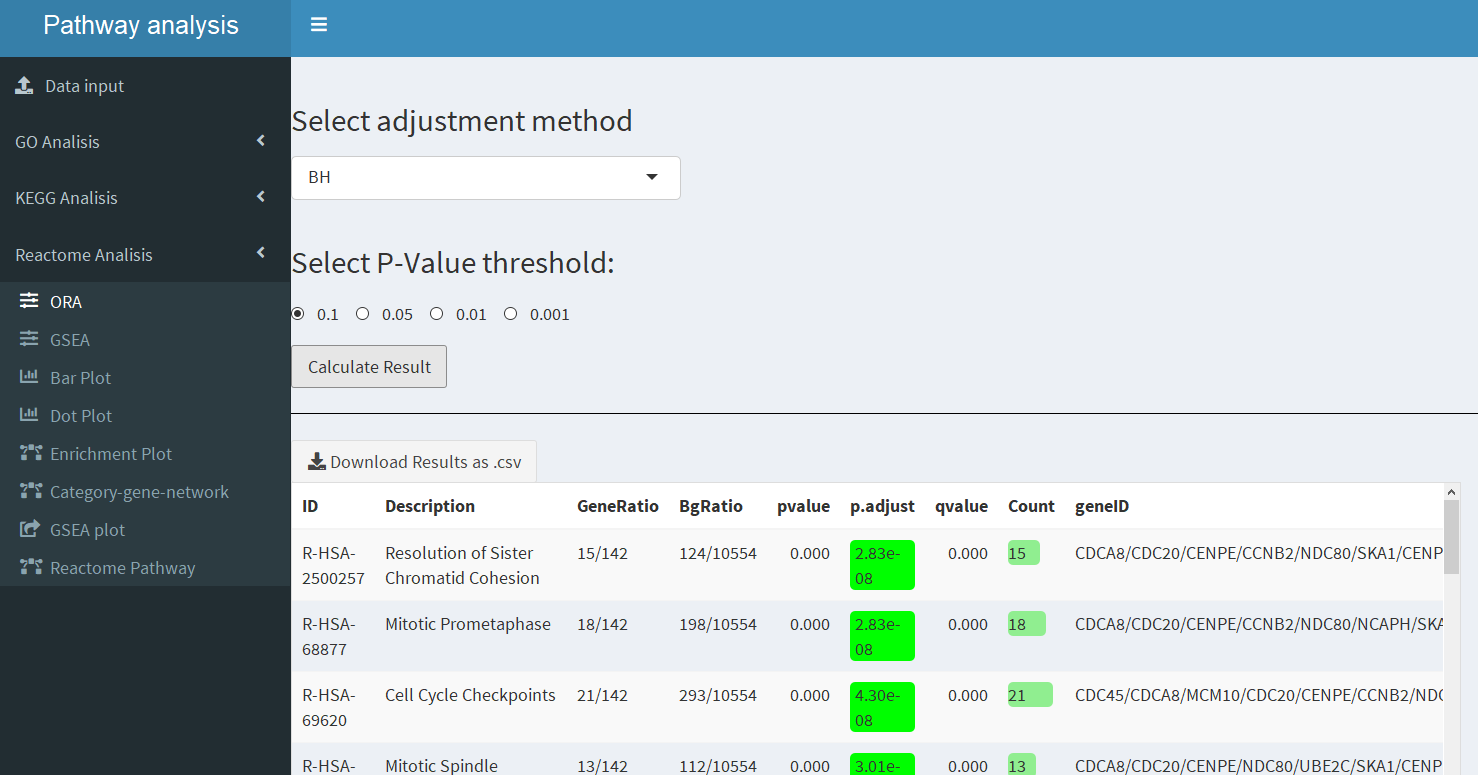
\includegraphics[width=0.9\textwidth]{App_F10_Items_Reactome_ORA.png} 
\caption{El resultat d'anàlisi ORA. Reactome.}
\end{figure}

\subsection{GSEA}
\subsubsection{GO}
El mètode GSEA per a termes GO es calcula amb la funció \helvetica{gseGO()} del paquet \helvetica{clusterProfiler}. 

\begin{lstlisting}[language=R]
gseGO(geneList, ont = "BP", OrgDb, keyType = "ENTREZID",
exponent = 1, nPerm = 1000, minGSSize = 10, maxGSSize = 500,
pvalueCutoff = 0.05, pAdjustMethod = "BH", verbose = TRUE,
seed = FALSE, by = "fgsea")
\end{lstlisting}

L'usuari pot elegir l'ontologia GO, el \textit{cut-off} del valor P i el mètode d'ajustament.
\begin{figure}[H]
\centering
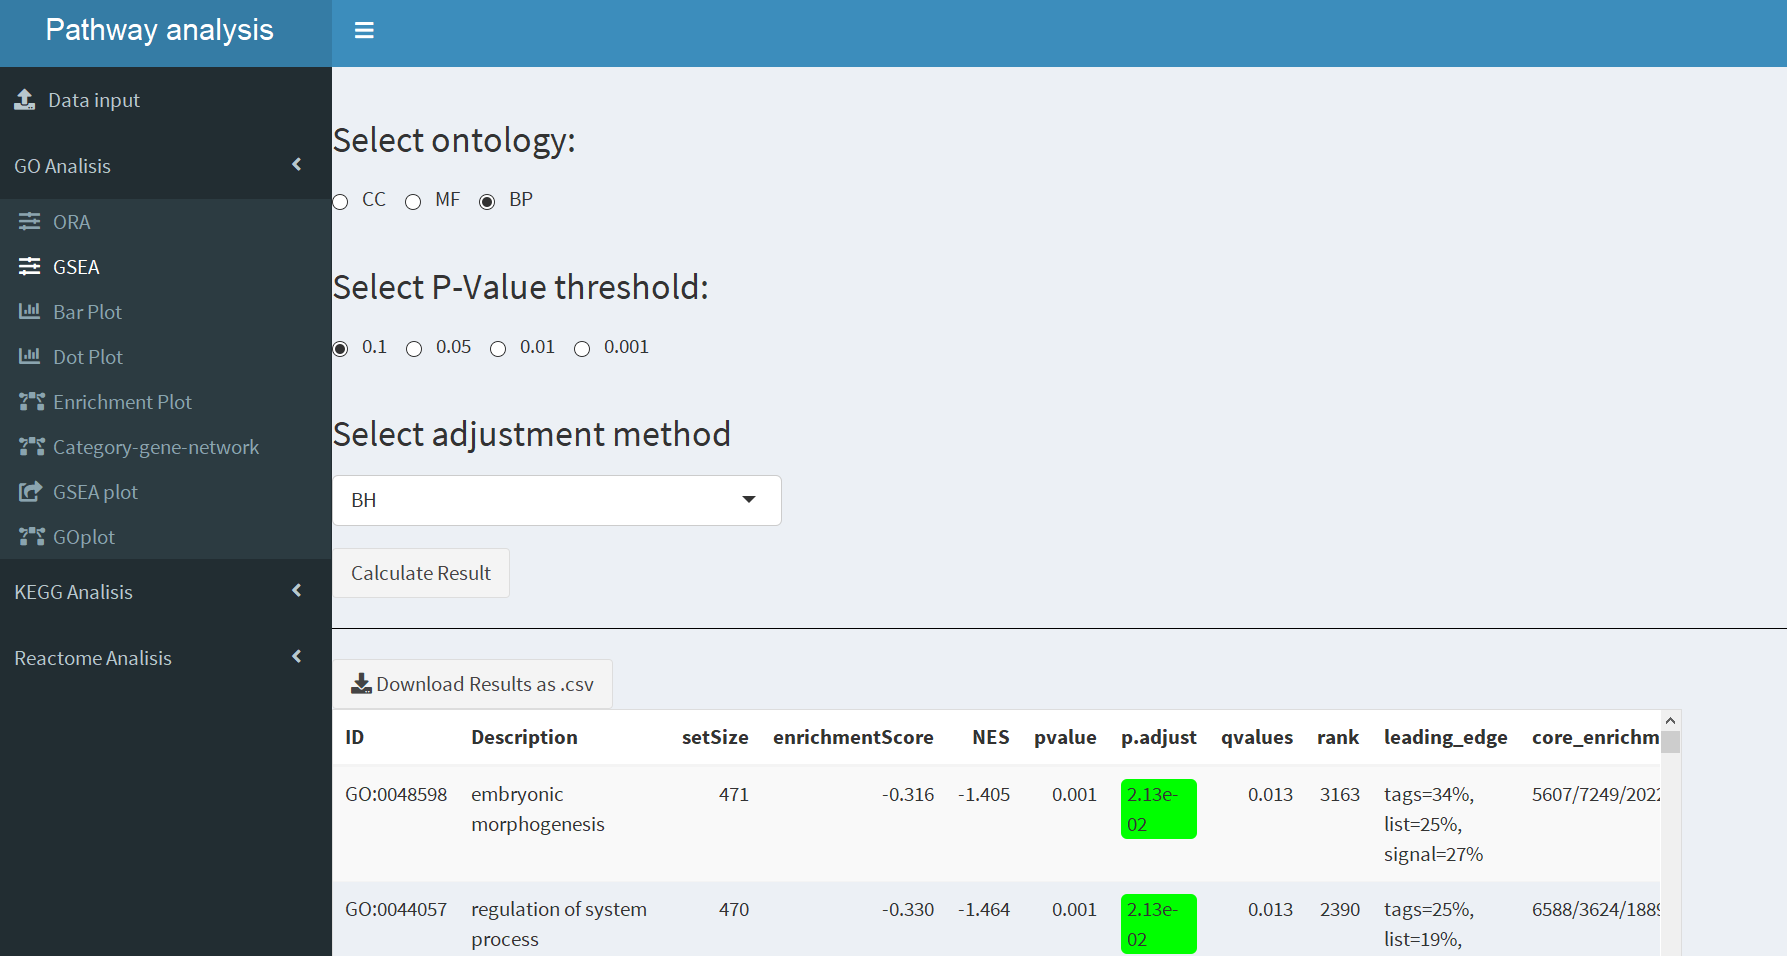
\includegraphics[width=0.9\textwidth]{App_F11_Items_GO_GSEA.png} 
\caption{El resultat de l'anàlisi GSEA. GO.}
\end{figure}

Per entendre l'anàlisi:



\begin{itemize}
\item \underline{enrichmentScore}. Enrichment score per al conjunt dels gens. Amb altres paraules: el grau amb el qual el conjunt dels gens està sobreexpressat a dalt o a baix del llistat ordenat dels gens en les dades d'expressió.
\item \underline{NES}. Normalized enrichment score. La puntuació per al conjunt de gens després de ser normalitzat tenint en compte tots els conjunts de gens analitzats (la seva mida i la seva correlació amb les dades d'expressió). Aquesta puntuació ajuda a comparar els resultats entre els conjunts de gens.
\item \underline{pvalue}.El valor de p nominal.
\item \underline{p.adjust}. El valor de p ajustat.
\item \underline{leading\_edge}
\begin{itemize}
\item \underline{Tags}. El percentatge de les ocurrències de gens del conjunt específic abans (per als ES positius) o després (per als ES negatius) del cim en la puntuació corrent d'enriquiment. Aquest valor indica el percentatge dels gens que contribueixen a la puntuació d'enriquement. 
\item \underline{List}. El percentatge dels gens en el llistat ordenat de tots els gens abans o després del pic en la puntuació corrent d'enriquiment. Aquest valor ens indica on exactament el pic es produeix. 
\item \underline{Signal}. La fortalesa del senyal d'enriquiment que combina els dos valors anteriors.
\end{itemize}
\item \underline{rank}. La posició del pic en la llista ordenada dels gens. Els conjunts dels gens més interessants assoleixen el seu màxim o bé al principi o al final de la llista ordenada. Vol dir que tenen aquest valor o bé molt baix o bé molt alt.
\end{itemize}

\subsubsection{KEGG}
De la mateixa manera es calcula GSEA amb la funció \helvetica{gseKEGG()} del paquet \helvetica{clusterProfiler}:

\begin{figure}[H]
\centering
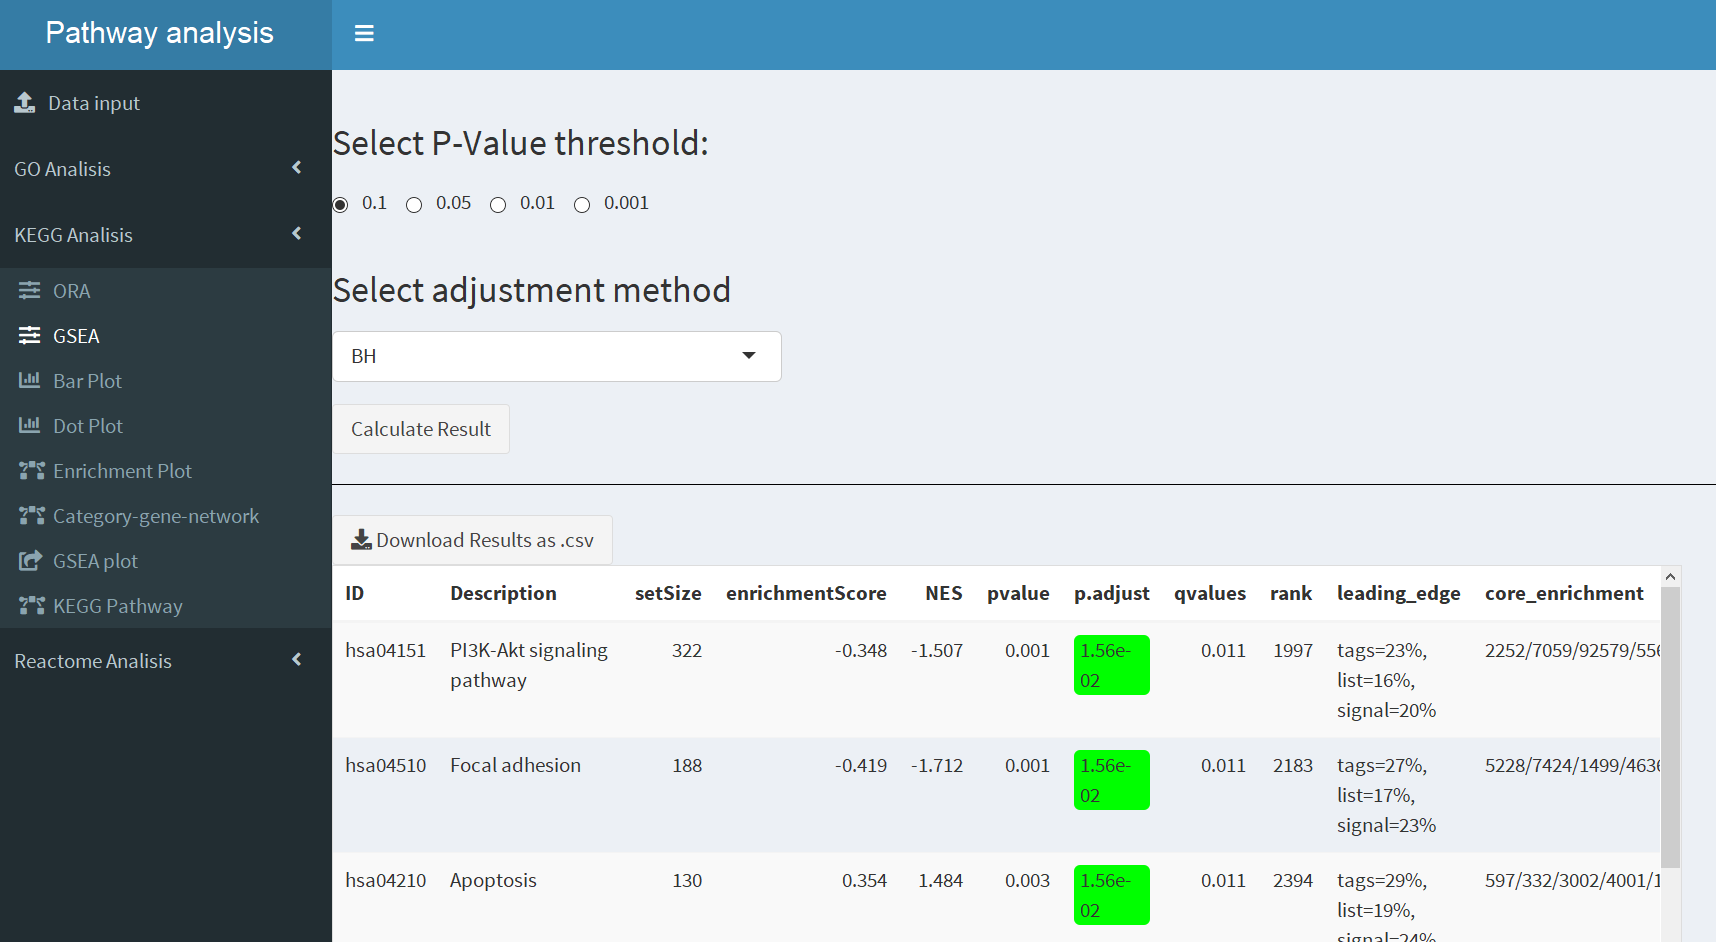
\includegraphics[width=0.9\textwidth]{App_F12_Items_KEGG_GSEA.png} 
\caption{El resultat de l'anàlisi GSEA. KEGG.}
\end{figure}

\subsubsection{Reactome}
Per completar l'anàlisi l'usuari pot calcular GSEA per a base de dades Reactome. Com als altres casos utilitzo el paquet \helvetica{clusterProfiler} i específicament la funció \helvetica{gsePathway()}

\begin{figure}[H]
\centering
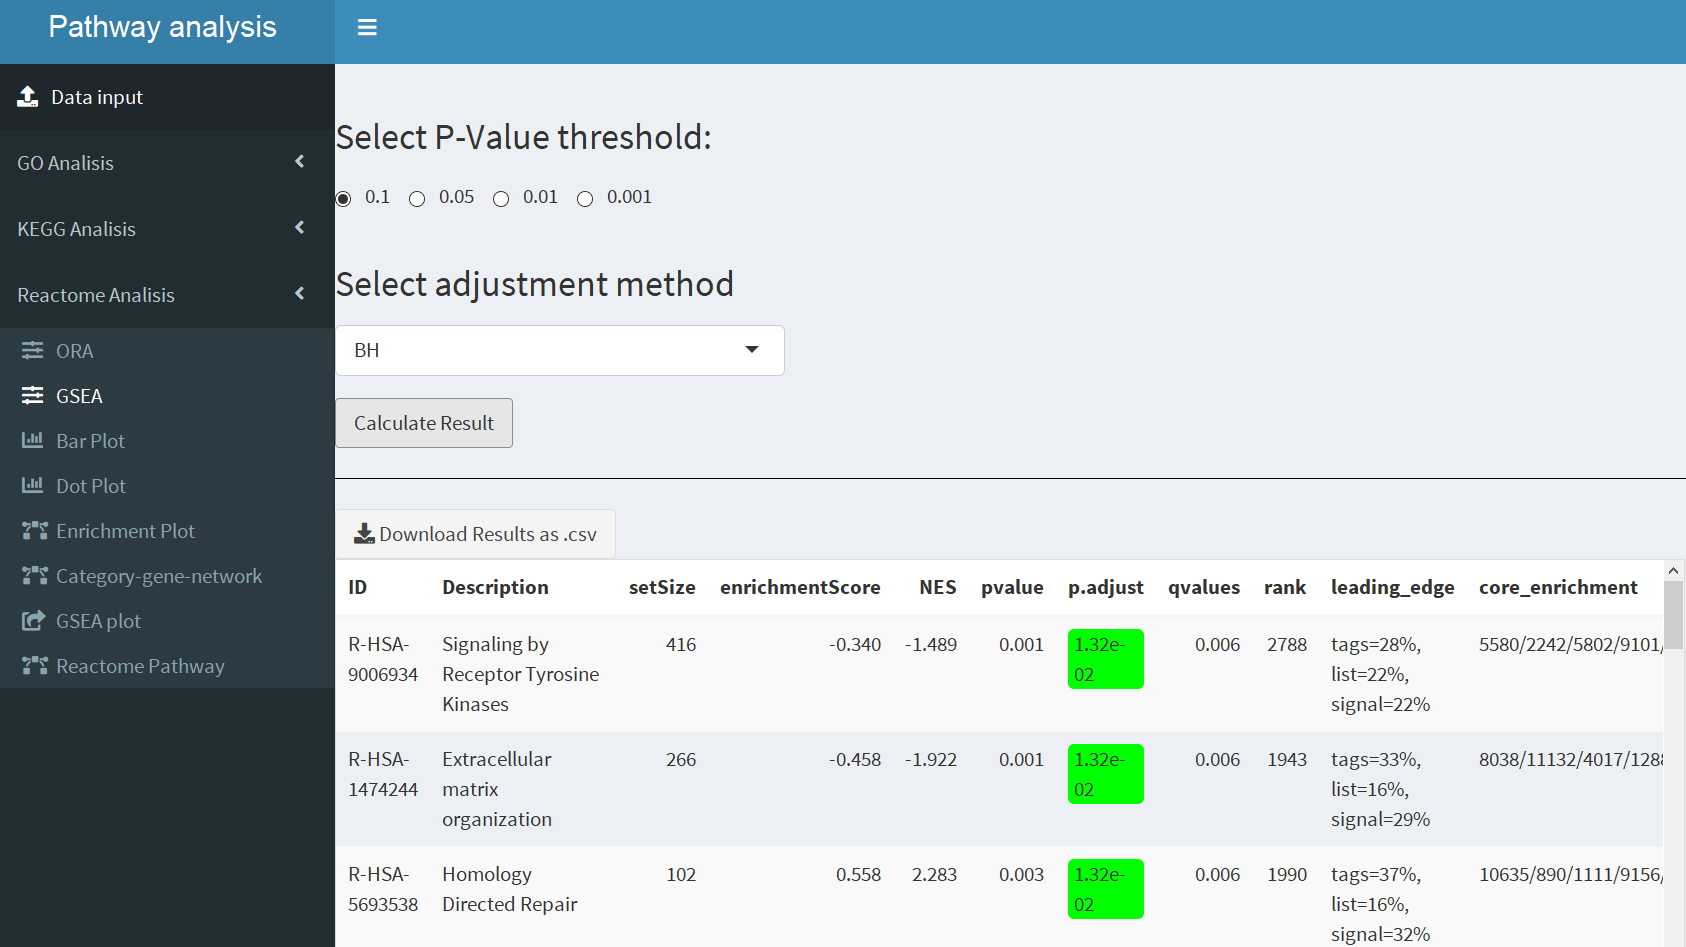
\includegraphics[width=0.9\textwidth]{App_F13_Items_RA_GSEA.png} 
\caption{El resultat d'anàlisi GSEA. Reactome.}
\end{figure}

\subsection{Bar-Plots}
Els resultats de \helvetica{enrichGO}, \helvetica{enrichKEGG} i \helvetica{enrichPathway} es poden visualitzar amb el gràfic de barres. L'usuari pot elegir el nombre de les categories visualitzades entre 2 i 30. Es dona l'opció per descarregar el gràfic en format .png.

\begin{figure}[H]
\centering
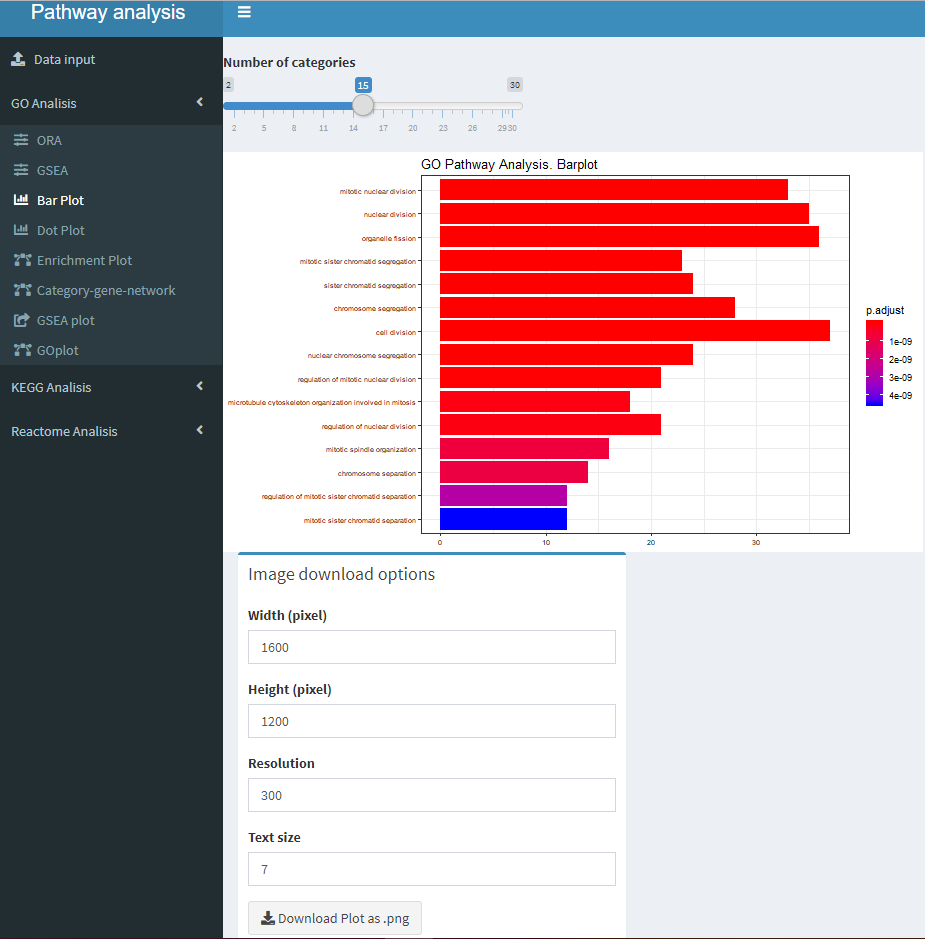
\includegraphics[width=0.9\textwidth]{App_F14_Items_GO_BarPlot.png} 
\caption{Bar-Plot. GO.}
\end{figure}

\subsection{Dot-Plots}

El \textit{dot plot} visualitza addicionalment el \textit{gen ratio}. També aquí l'usuari pot seleccionar el nombre de categories.


\begin{figure}[H]
\centering
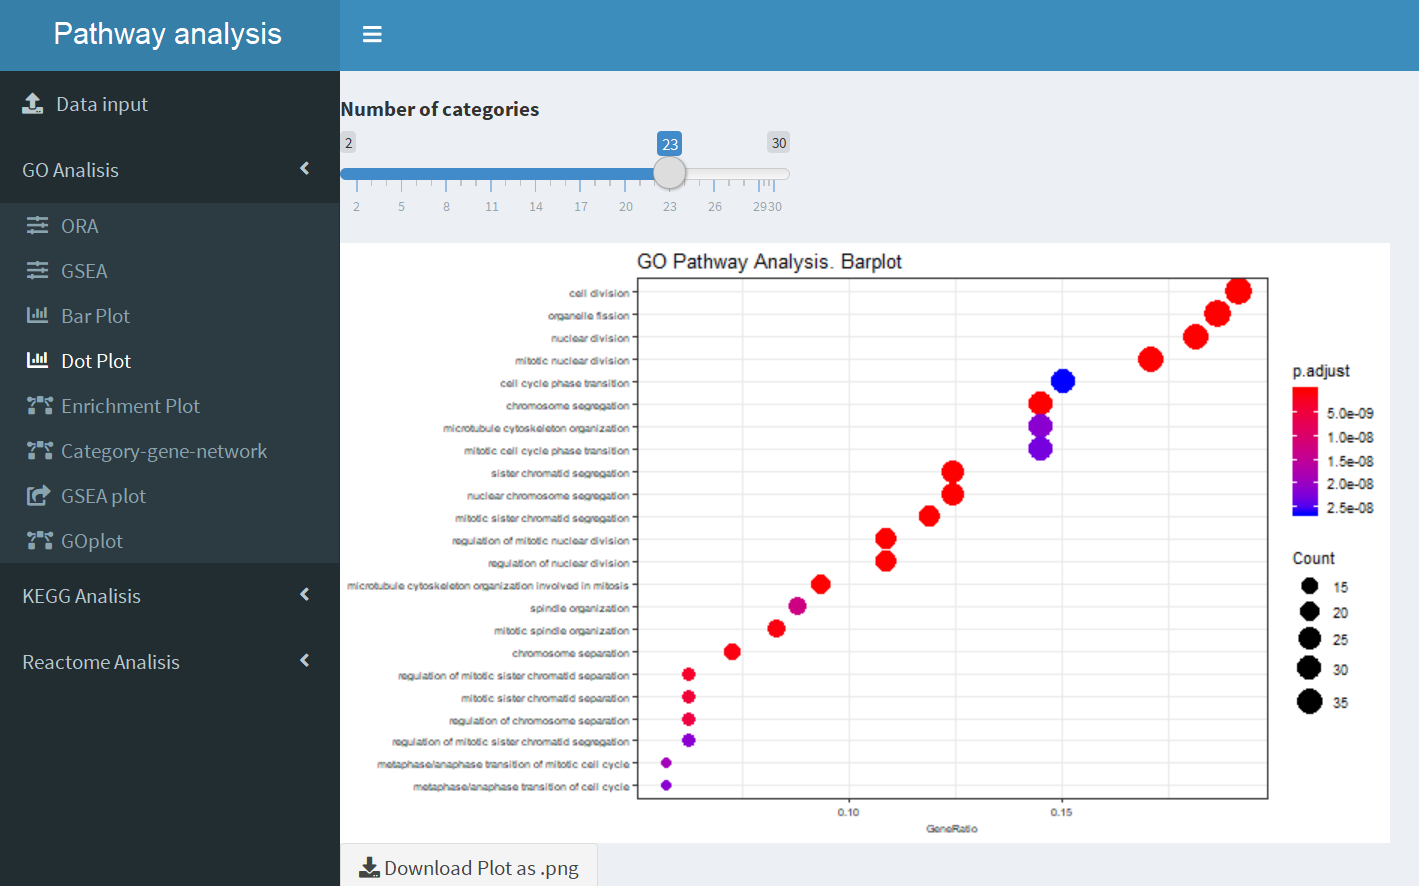
\includegraphics[width=0.9\textwidth]{App_F15_Items_GO_DotPlot.png} 
\caption{Bar-Plot. GO.}
\end{figure}

\subsection{Enrichment Plots}

\begin{figure}[H]
\centering
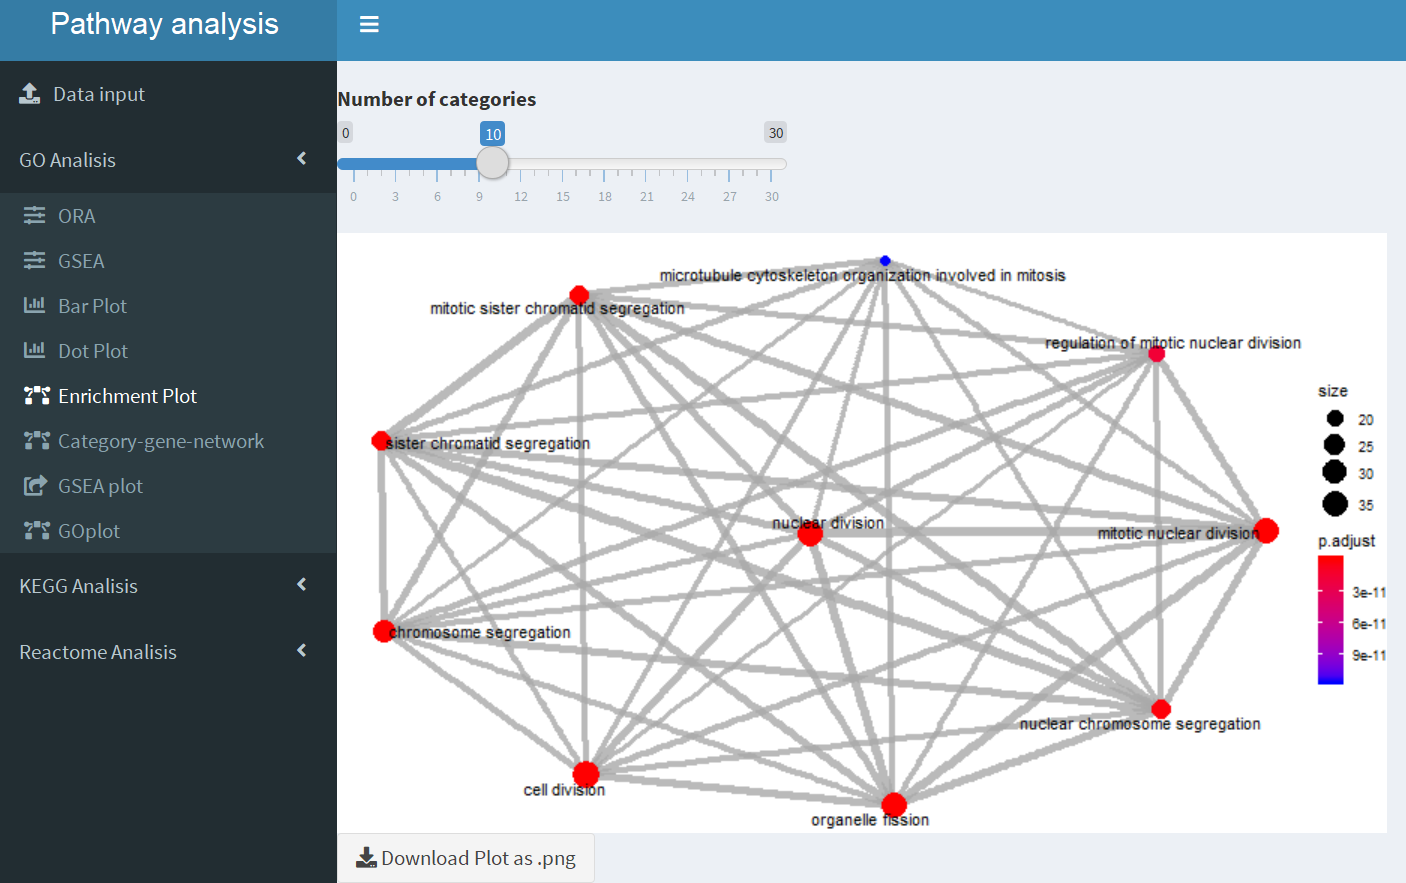
\includegraphics[width=0.9\textwidth]{App_F16_Items_GO_Emap.png} 
\caption{Bar-Plot. GO.}
\end{figure}

\subsection{Category-Gene-Network Plot}

\begin{figure}[H]
\centering
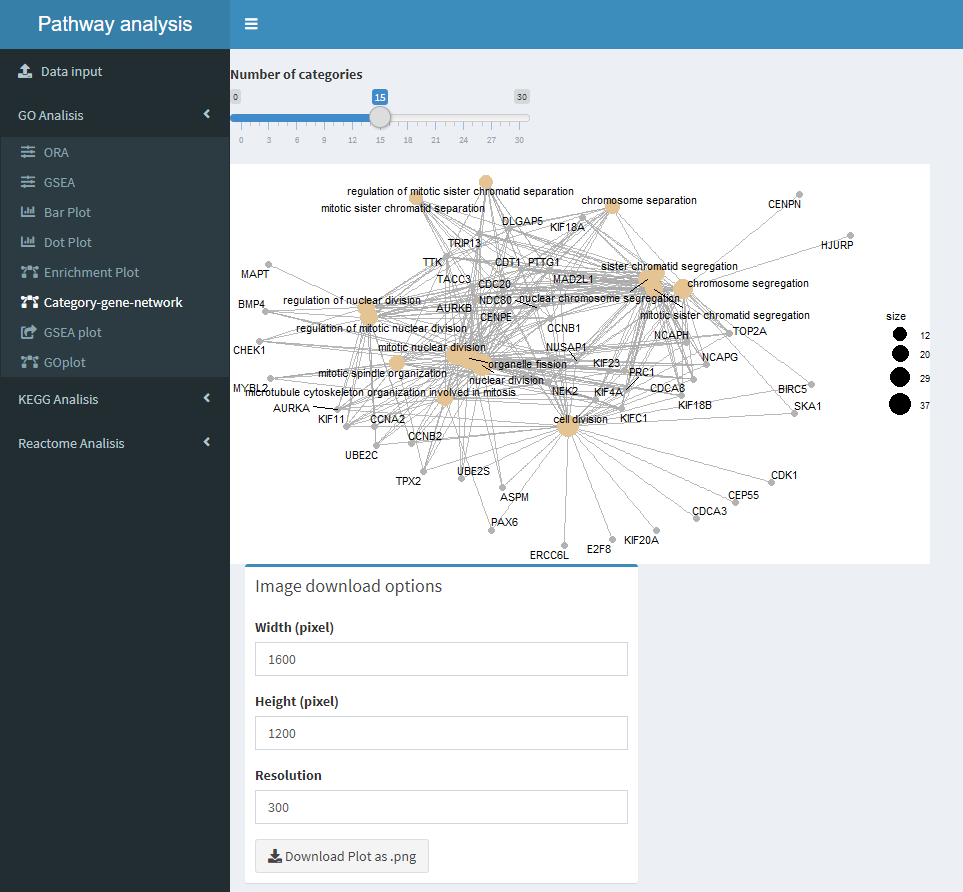
\includegraphics[width=0.9\textwidth]{App_F17_Items_GO_CnetPlot.png} 
\caption{Category-Gene-Network Plot. GO.}
\end{figure}

\subsection{GSEA Plot}
L'usuari pot visualitzar una de les categories disponibles via \textit{dropdown list}. El llistat inclou totes les rutes generades durant l'anàlisi GSEA en els apartats \textit{Go Analysis}$\rightarrow$\textit{GSEA}; \textit{KEGG}$\rightarrow$\textit{GSEA}
\begin{figure}[H]
\centering
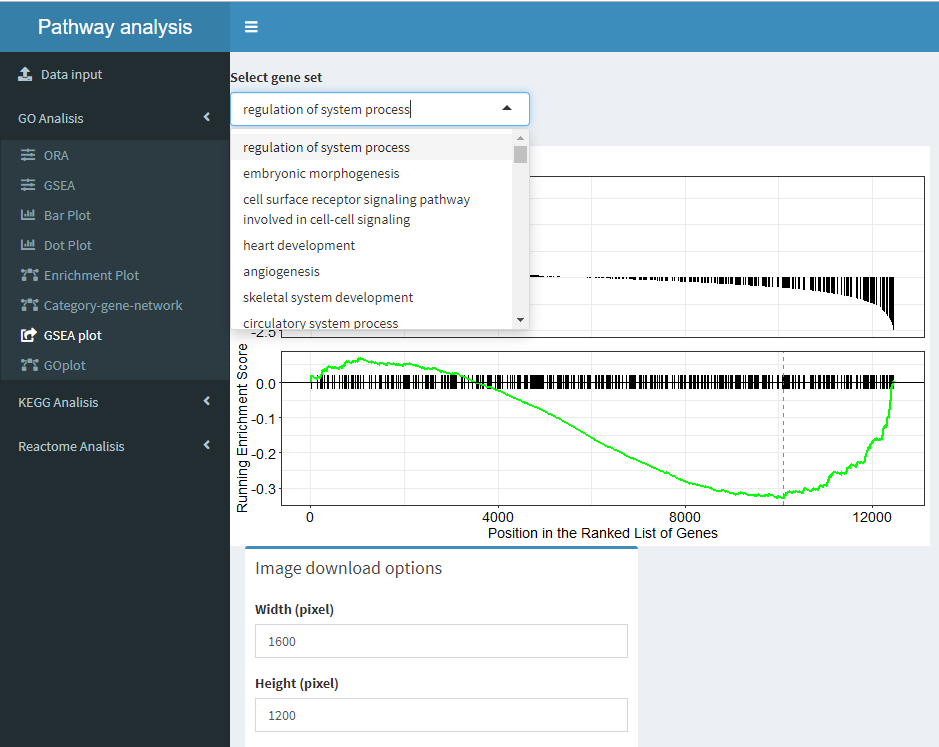
\includegraphics[width=0.9\textwidth]{App_F18_Items_GO_GSEA_Plot.png} 
\caption{GSEA Plot. GO.}
\end{figure}


\section{L'anàlisi específic de GO, KEGG i Reactome}

\label{sec:ASpec}


\subsection{GO Plot}

\begin{figure}[H]
\centering
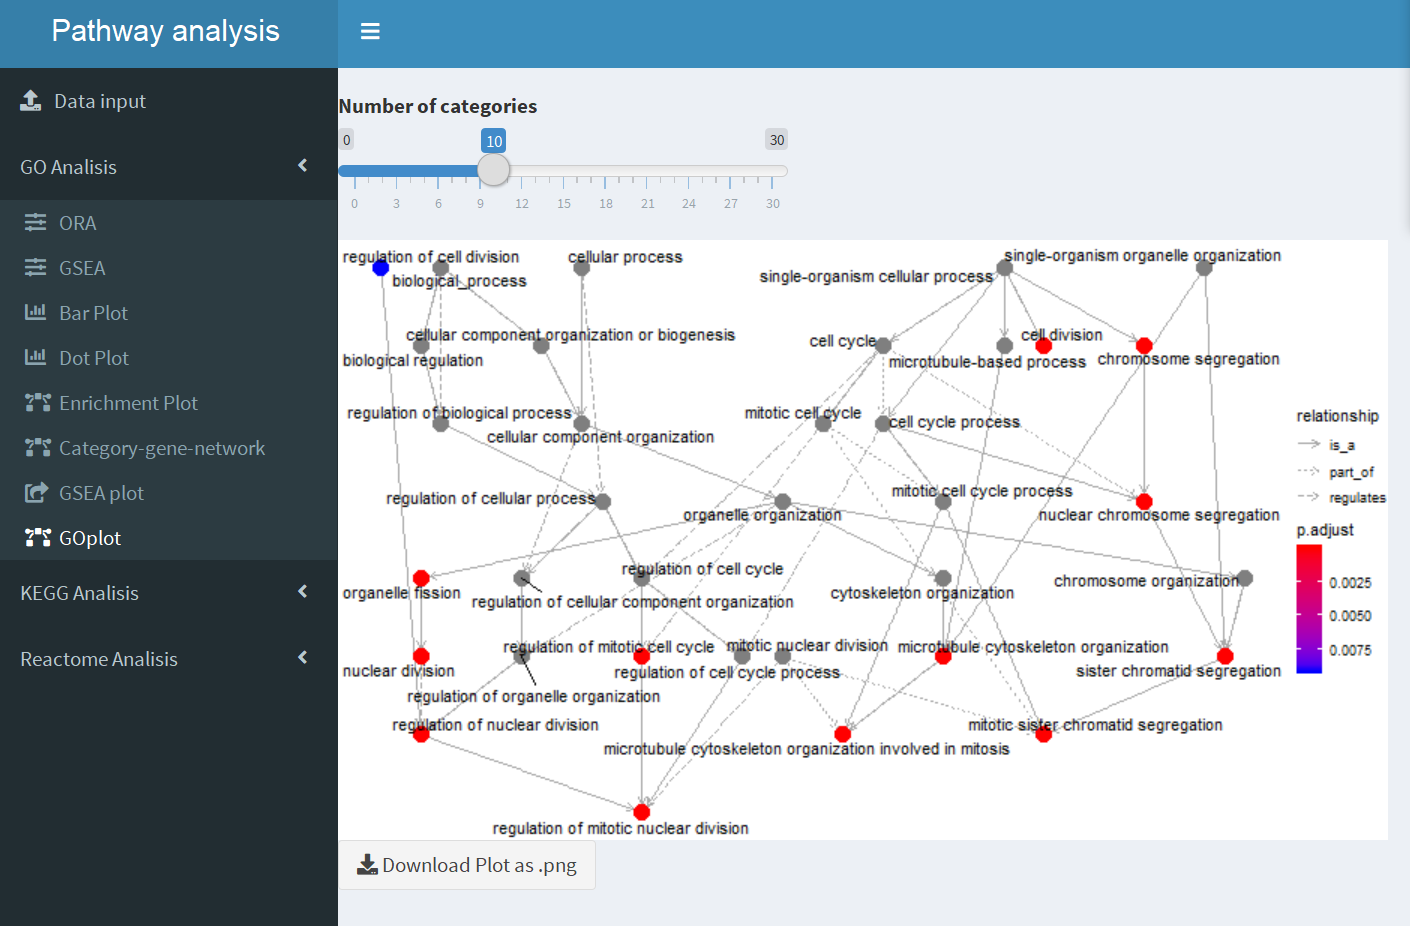
\includegraphics[width=0.9\textwidth]{App_F19_Items_GO_GOPlot.png} 
\caption{GO Plot}
\end{figure}

\subsection{KEGG Pathway}


\begin{figure}[H]
\centering
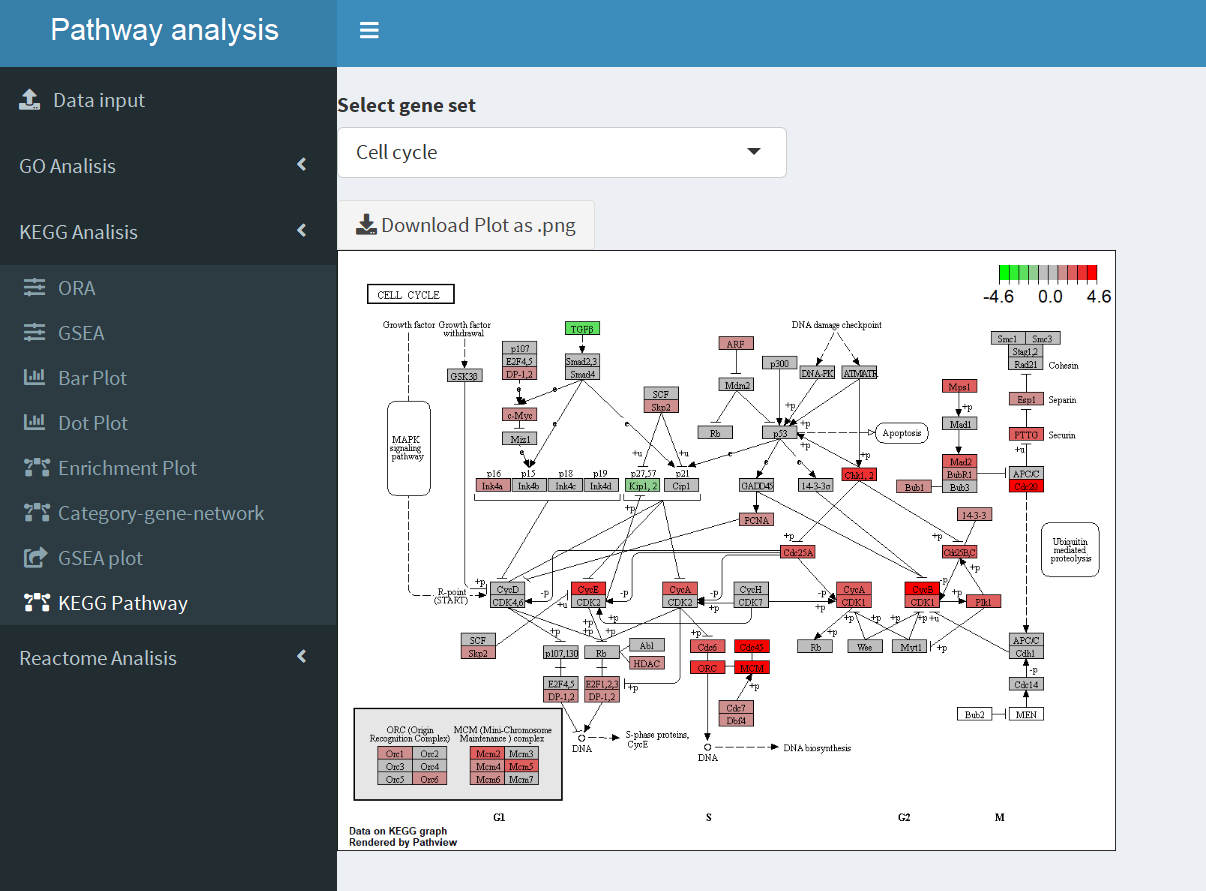
\includegraphics[width=0.9\textwidth]{App_F20_Items_KEGG_KEGGPathway.png} 
\caption{KEGG pathway}
\end{figure}

\subsection{Reactome Pathway}

\begin{figure}[H]
\centering
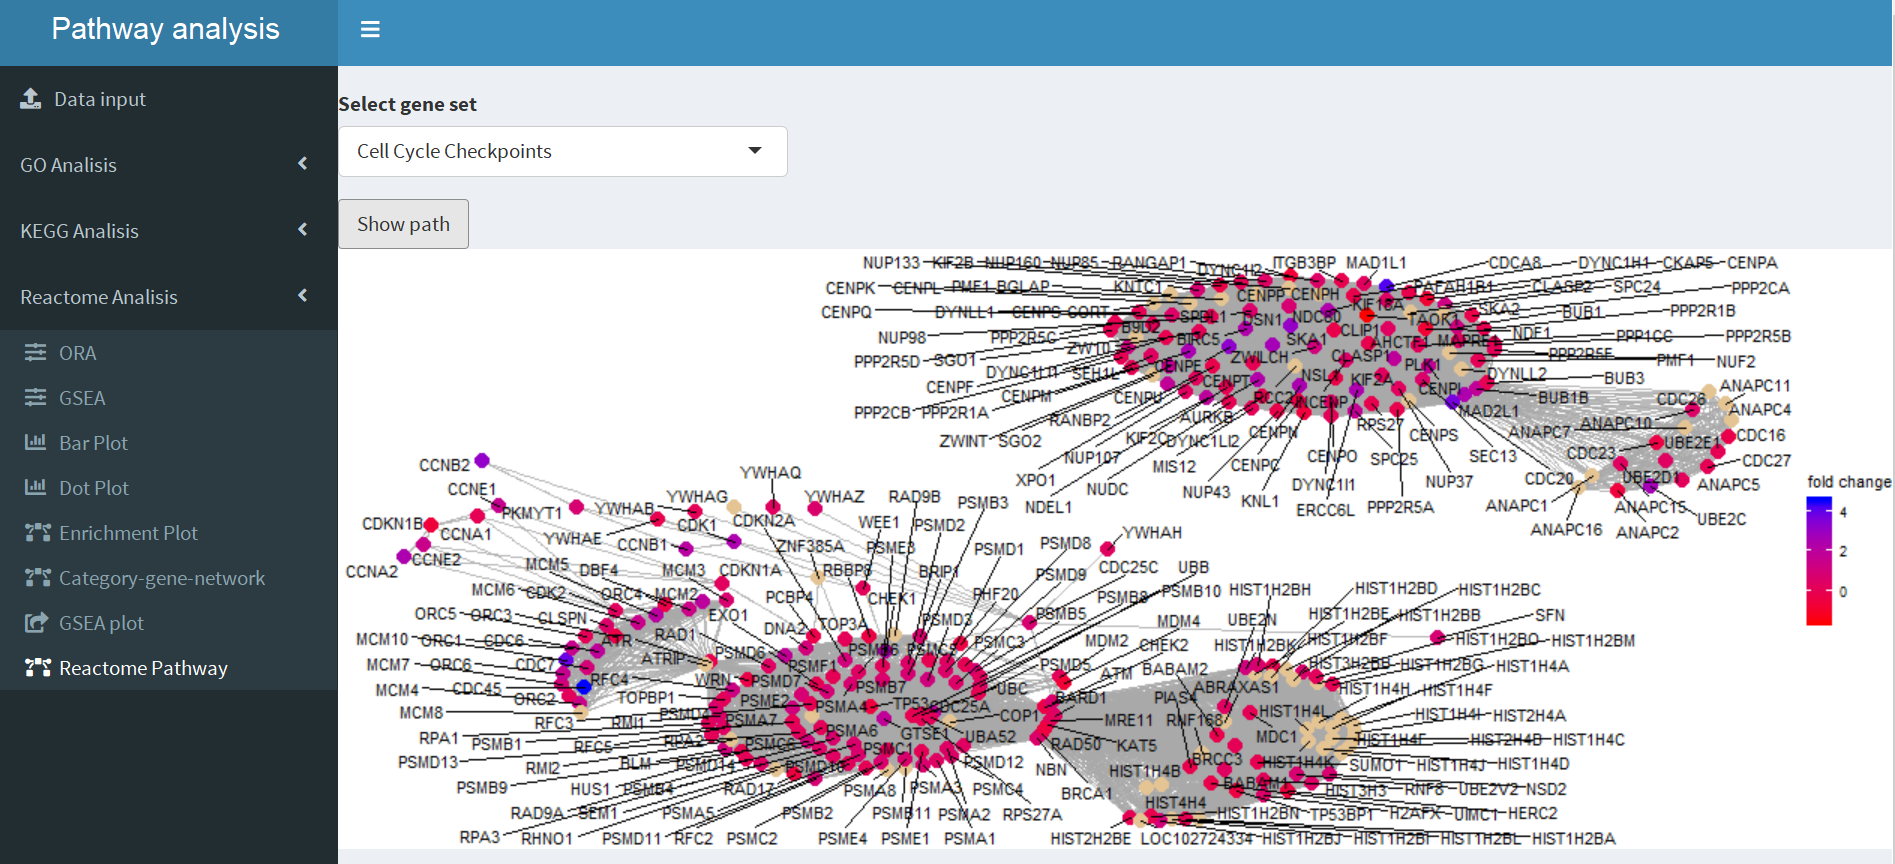
\includegraphics[width=0.9\textwidth]{App_F21_Items_RA_RAPathway.png} 
\caption{Reactome pathway}
\end{figure}


\section{Validació dels resultats}
\label{sec:ValRes}

L’anàlisi de les rutes representa l’últim pas de l’anàlisi d’expressions. Per dur a terme l’anàlisi de rutes és necessari tenir unes dades que ja estiguin processades prèviament (normalització, càlcul de les LogRatios, ajustament dels gens repetits a l’array, selecció dels gens diferencialment expressats, etc.). Les dades de \href{https://www.ncbi.nlm.nih.gov/geo/}{GEO (Gene Expression Omnibus)} estan però disponibles com a màxim en format normalitzat. Caldria doncs fer una anàlisi per arribar a un llistat de gens diferencialment expressats amb les logRatios per tots els gens de la mostra. Fer això no seria cap problema i de fet ho he fet per altres estudis. El problema és que arribo a resultats diferents dels resultats dels estudis d’on provenen les dades (i no parlo de l’anàlisi de les rutes sinó ja del càlcul de les logRatios). Per tant les dades que entraria a l’aplicació serien diferents de les dades de l’estudi i lògicament amb aquesta comprovació no comprovo el que realment m’interessa. Podria, doncs, dedicar-me a trobar el motiu pel qual els resultats són diferents, però fer totes aquestes comprovacions prèvies no té a veure amb l’objecte del meu treball de màster, l’anàlisi de les rutes. Per tant he procedit a contactar el meu profesor per si tindria (o coneixeria) dades preprocessades fins a un llistat de gens amb logRatios i amb el set de gens diferencialment expressats, per tal que les pugui utilitzar en la meva aplicació. El meu professor m'ha redirigit, entre altres enllaços molt útils, al seu repositori en \href{https://github.com/alexsanchezpla?tab=repositories}{github.com}. 


\begin{center}
\begin{tabular}{||c | c | c | c | c ||} 
\hline 
Estudi & GEO ID & Espècie & Tipo d'experiment & Font \\ [0.5ex] 
\hline\hline
\cite{schmidt2008humoral} & \href{https://www.ncbi.nlm.nih.gov/geo/query/acc.cgi?acc=GSE11121}{GSE11121}& Homo sapiens & Microarrays & \href{https://bioconductor.org/packages/release/bioc/html/DOSE.html}{Paquet \helvetica{DOSE} de Bioconductor}\\
\hline
\cite{li2017zbtb7b} & \href{https://www.ncbi.nlm.nih.gov/geo/query/acc.cgi?acc=GSE100924}{GSE100924}& Mus musculus & Microarrays & \href{https://github.com/alexsanchezpla/StatisticalAnalysisOfMicroarrayData}{Github Sanchez Pla} \\ 
\hline
\cite{farmer2005identification} & \href{https://www.ncbi.nlm.nih.gov/geo/query/acc.cgi?acc=GSE1561}{GSE1561}&Homo sapiens& Microarrays & \href{https://github.com/alexsanchezpla/Ejemplo_de_MDA_con_Bioconductor}{Github Sanchez Pla} \\ 
\hline
\cite{hengel2003cutting} & \href{https://david.ncifcrf.gov/helps/demo1.txt}{DAVID Demo List 1}&Homo sapiens& Microarrays & \href{https://david.ncifcrf.gov/content.jsp?file=FAQs.html}{DAVID} \\ 
\hline
\end{tabular}
\end{center}

Les dades de \cite{schmidt2008humoral}, que s'utilitzen en els vignettes de \helvetica{clusterProfiler} i \helvetica{ReactomePA}, ja les he mostrat en gran part a dalt quan explicava el contingut de l'aplicació. Els resultats obtinguts amb l'aplicació són iguals als resultats en els vignettes mencionats. Procediré doncs amb l'exemple basat en les dades de \cite{li2017zbtb7b} .

\subsection{Exemple d'anàlisi 1. GEO: GSE100924}

Les dades d'estudi \cite{li2017zbtb7b} són ja preprocessades per Ricardo Gonzalo Sanz i Sanchez Pla i estan disponibles a \href{https://github.com/alexsanchezpla/StatisticalAnalysisOfMicroarrayData}{github}. De la carpeta \textit{results} he agafat la taula \textit{topAnnotated\_KOvsWT\_COLD.csv}. Sanz i Pla utilitzen el paquet \helvetica{ReactomePA} per a l'anàlisi d'enriquiment. Repeteixo doncs el seu anàlisi utilitzant l'aplicació. 

\begin{enumerate}

\item Ellegeixo l'espècie \textit{Mus musculus} per a GO, KEGG i Reactome.
\begin{figure}[H]
\centering
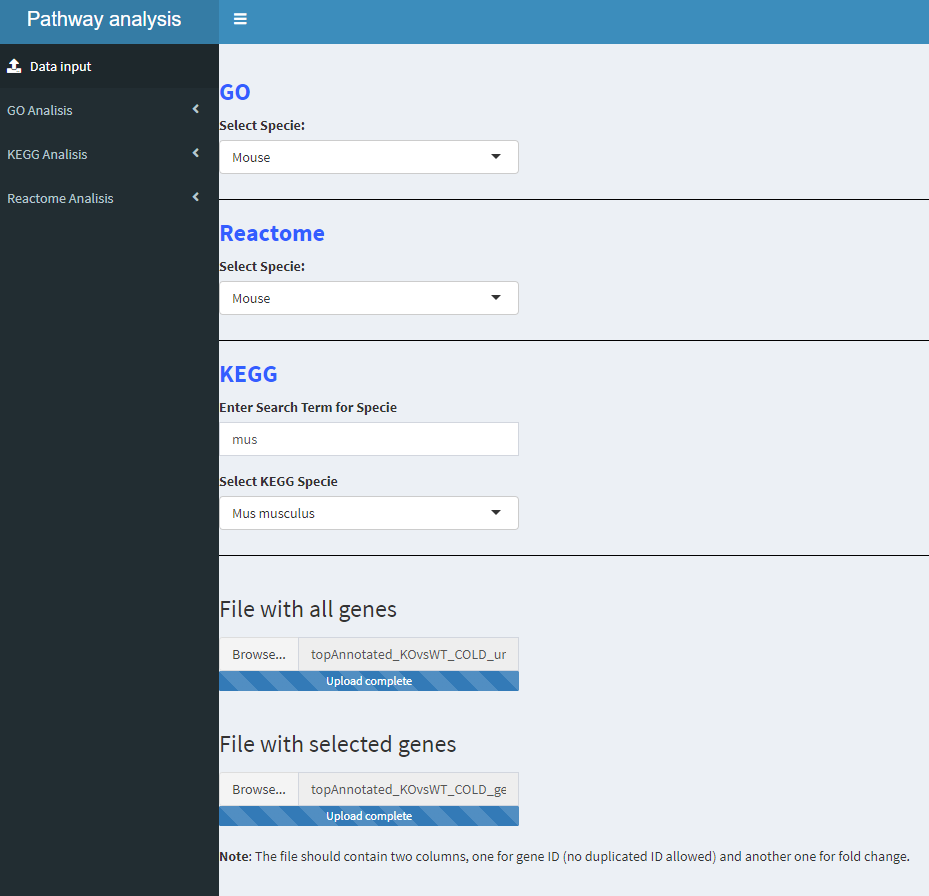
\includegraphics[width=0.6\textwidth]{Estudi1_Fig1_Select_Specie.png} 
\caption{Selecció d'espècie}
\end{figure}

L'output a baix indica que s'ha pujat el total de 5995 gens. Per a l'arxiu dels gens seleccionats l'aplicació diu que s'han pujat 769 gens.

\begin{figure}[H]
\centering
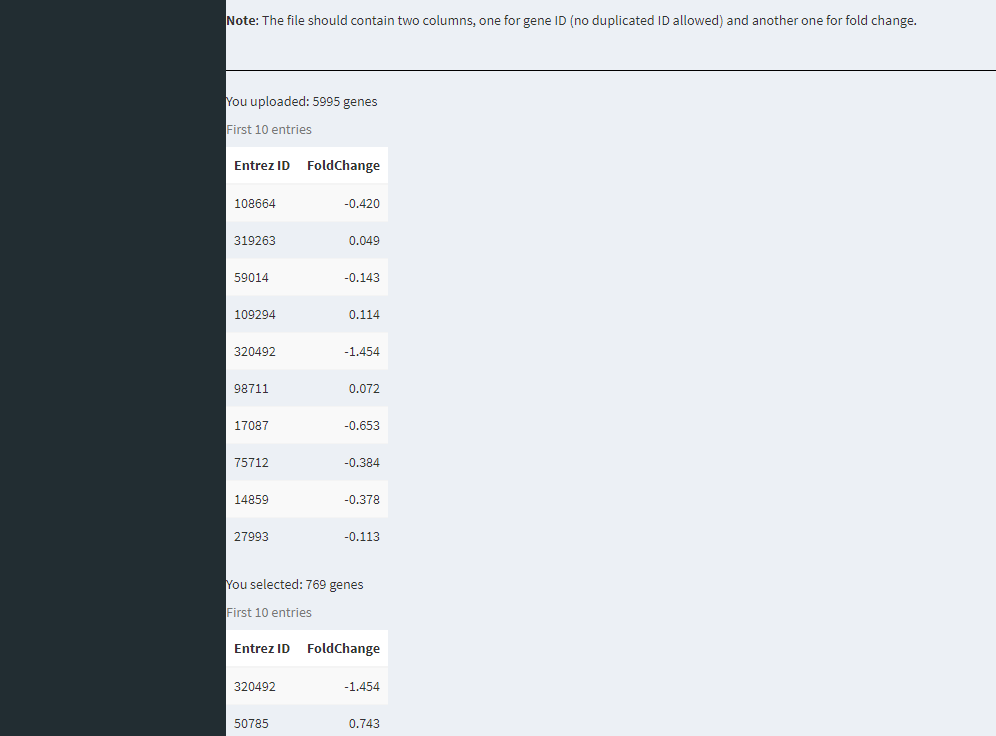
\includegraphics[width=0.6\textwidth]{Estudi1_Fig2_Select_Specie.png} 
\caption{Selecció d'espècie}
\end{figure}


\item Clico en l'apartat \textit{Reactome Analysis}$\rightarrow$\textit{ORA}. Selecciono com a mètode d'ajustament \textit{BH} i el cut-off del valor de P ajustat 0.05. Clico a \textit{Calculate results}

\begin{figure}[H]
\centering
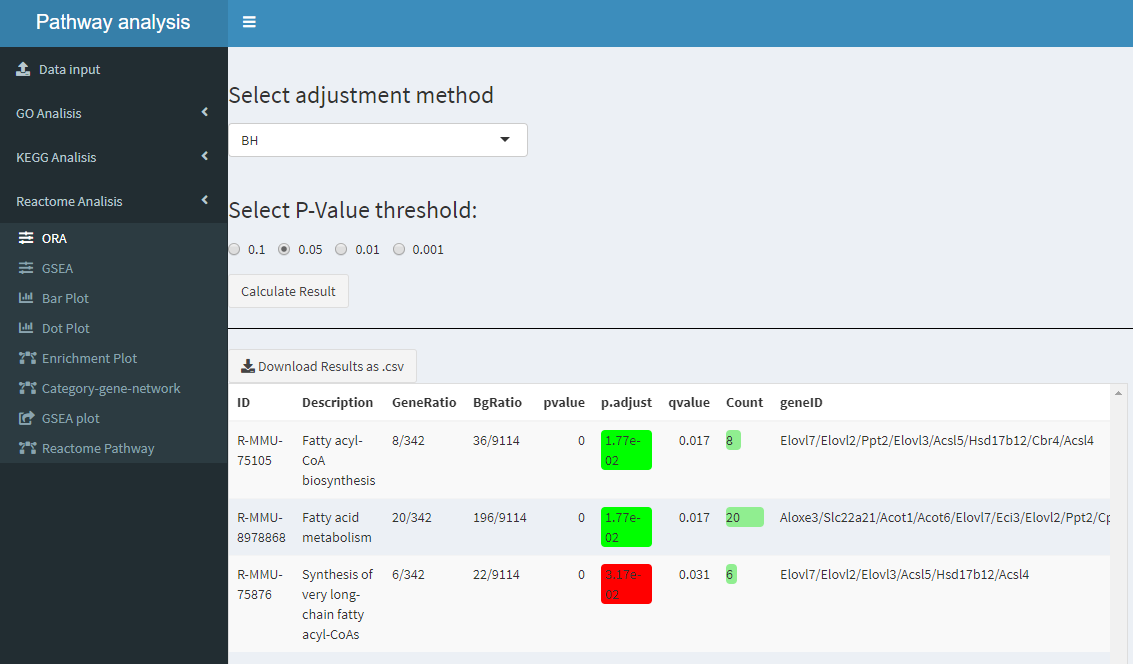
\includegraphics[width=0.6\textwidth]{Estudi1_Fig3_ORA_RA.png} 
\caption{Resultat d'anàlisi ORA de Reactome}
\end{figure}

Observem que els gens mostrats són els mateixos esmentats per Sanz i Pla.

\item Visualització del resultat ORA

\begin{itemize}
\item Selecciono \textit{Reactome Analysis}$\rightarrow$\textit{Bar Plot}

\begin{figure}[H]
\centering
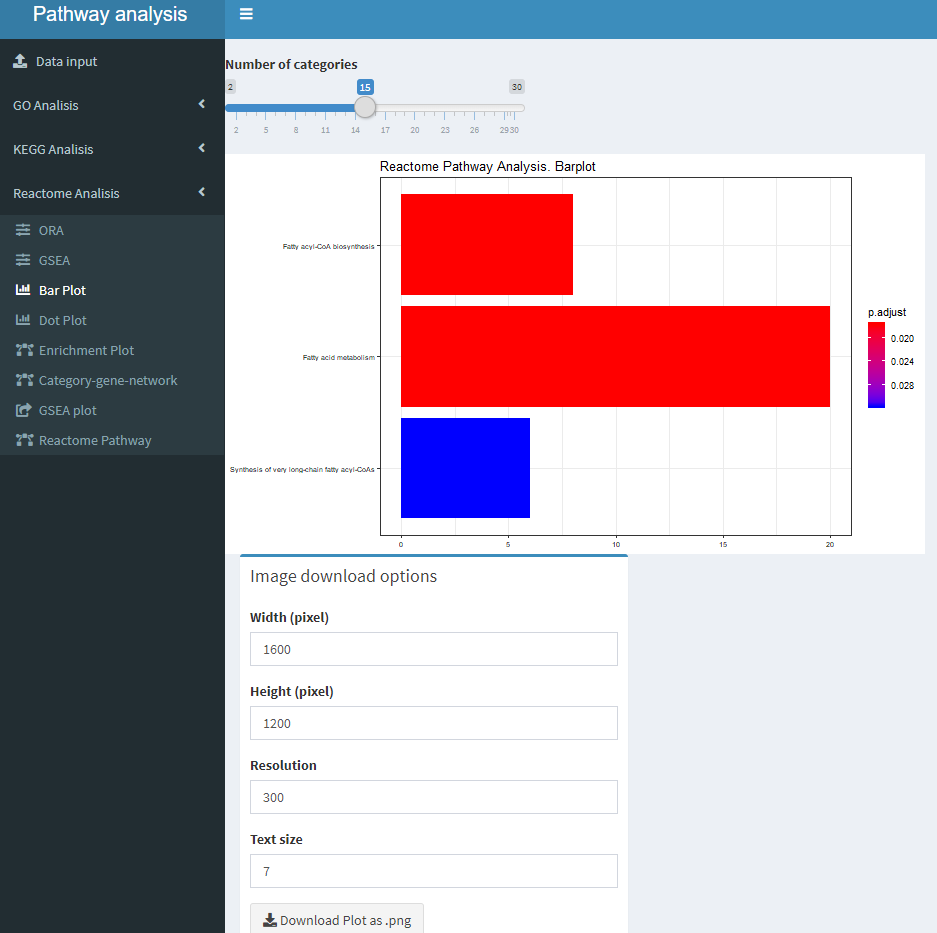
\includegraphics[width=0.6\textwidth]{Estudi1_Fig4_ORA_BP_RA.png} 
\caption{Gràfic de barres}
\end{figure}

\item Selecciono \textit{Reactome Analysis}$\rightarrow$\textit{Dot Plot}

\begin{figure}[H]
\centering
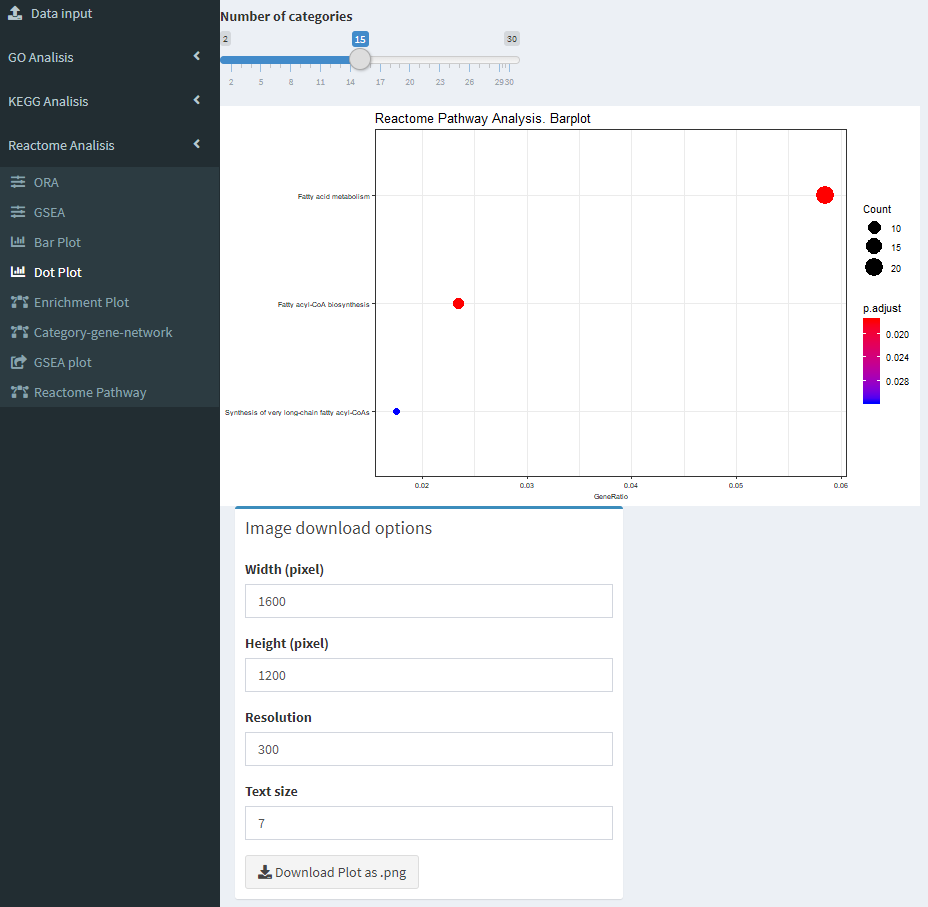
\includegraphics[width=0.6\textwidth]{Estudi1_Fig5_ORA_Dot_RA.png} 
\caption{Gràfic de punts}
\end{figure}

\item Selecciono \textit{Reactome Analysis}$\rightarrow$\textit{Enrichment Map Plot}

\begin{figure}[H]
\centering
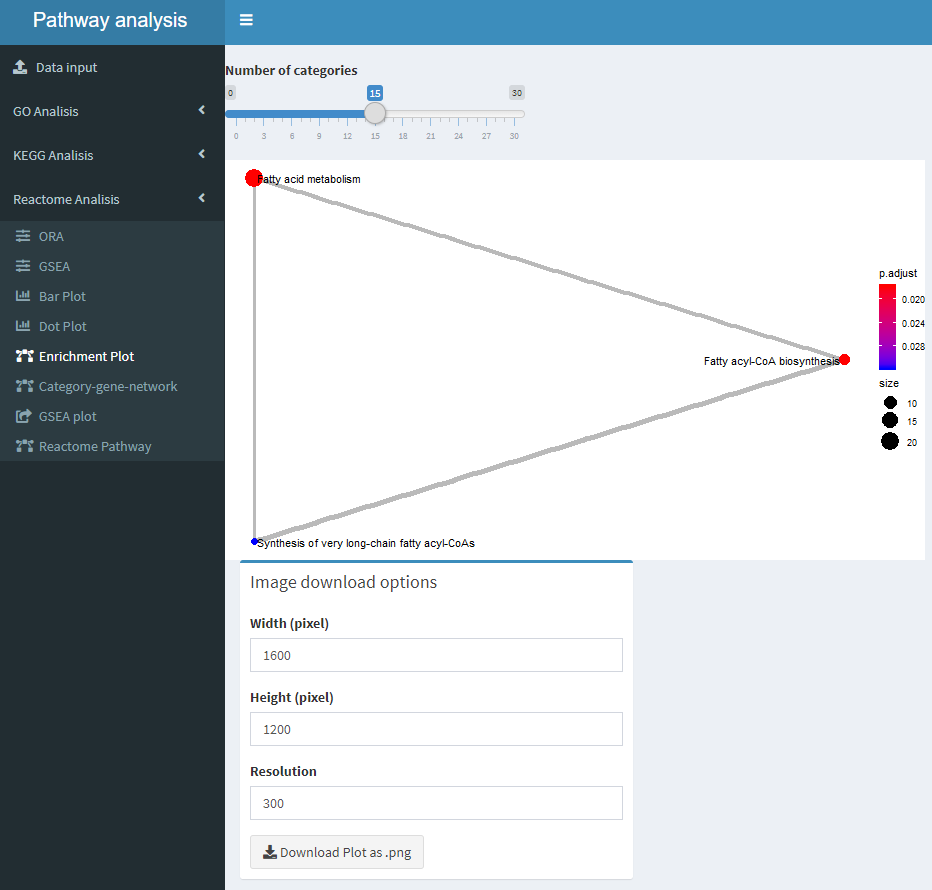
\includegraphics[width=0.6\textwidth]{Estudi1_Fig6_ORA_EP_RA.png} 
\caption{Mapa d'enriquement}
\end{figure}

\item Selecciono \textit{Reactome Analysis}$\rightarrow$\textit{Category Gene Network}
\begin{figure}[H]
\centering
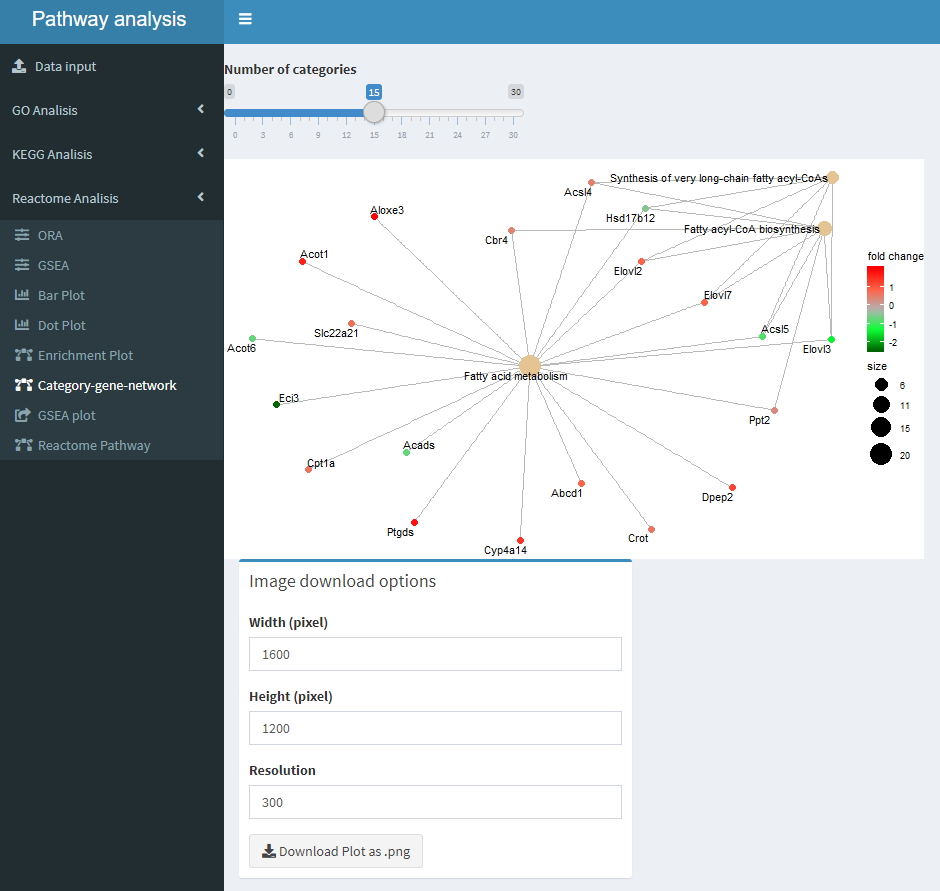
\includegraphics[width=0.6\textwidth]{Estudi1_Fig7_ORA_CP_RA.png} 
\caption{Red de les categories i gens}
\end{figure}

\item Selecciono \textit{Reactome Analysis}$\rightarrow$\textit{Reactome Pathway}
\begin{figure}[H]
\centering
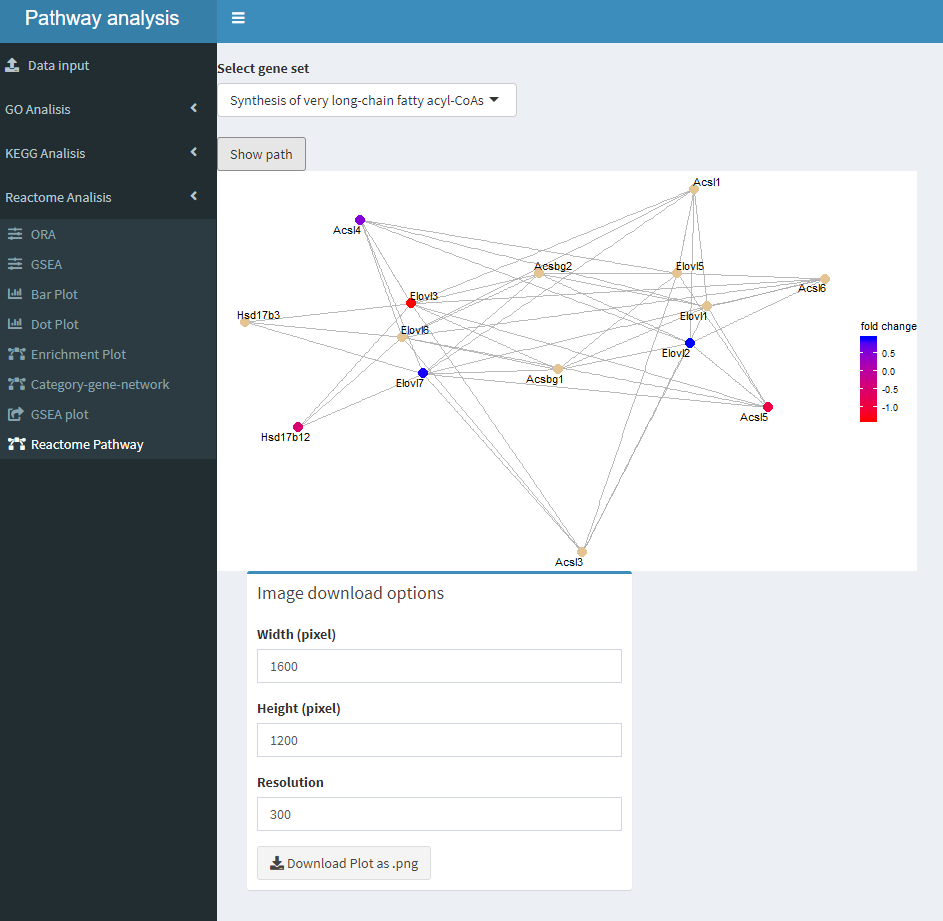
\includegraphics[width=0.6\textwidth]{Estudi1_Fig8_ORA_PP_RA.png} 
\caption{Rutes Reactome}
\end{figure}
\end{itemize}
\end{enumerate}

Addicionalment a l'anàlisi ORA podem fer, mitjançant l'aplicació, l'anàlisi GSEA per les rutes de Reactome. Per fer-ho:

\begin{enumerate}

\item Clico en l'apartat \textit{Reactome Analysis}$\rightarrow$\textit{GSEA}. Selecciono com a mètode d'ajustament \textit{BH} i el cut-off del valor de P ajustat 0.05. Clico a \textit{Calculate results}

Amb el valor de P de 0.05 l'anàlisi no troba cap ruta enriquida.

\item Augmento el Cut-Off del valor de P a 0.1

Amb el Cut-Off més alt l'aplicació retorna un llistat de gens.

\begin{figure}[H]
\centering
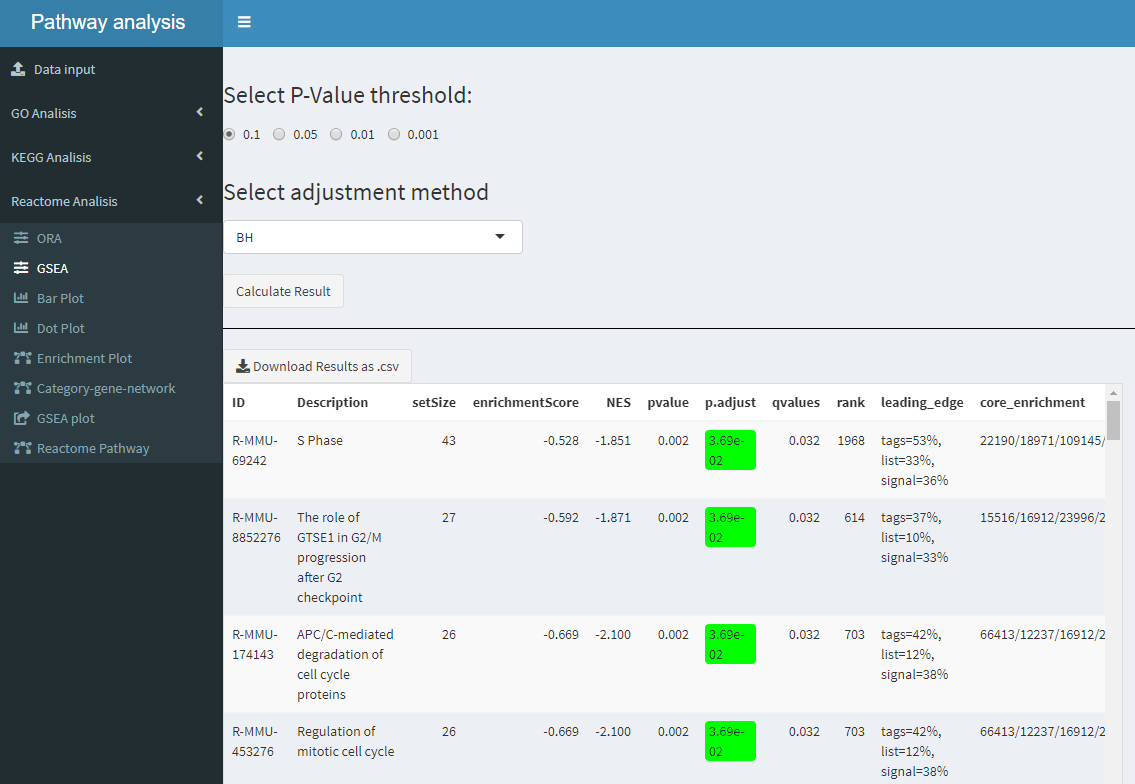
\includegraphics[width=0.6\textwidth]{Estudi1_Fig9_GSEA_RA.png} 
\caption{Anàlisi GSEA}
\end{figure}

\item Per obtenir els gràfics GSEA anem a \textit{Reactome Analysis}$\rightarrow$\textit{GSEA plot}

\begin{figure}[H]
\centering
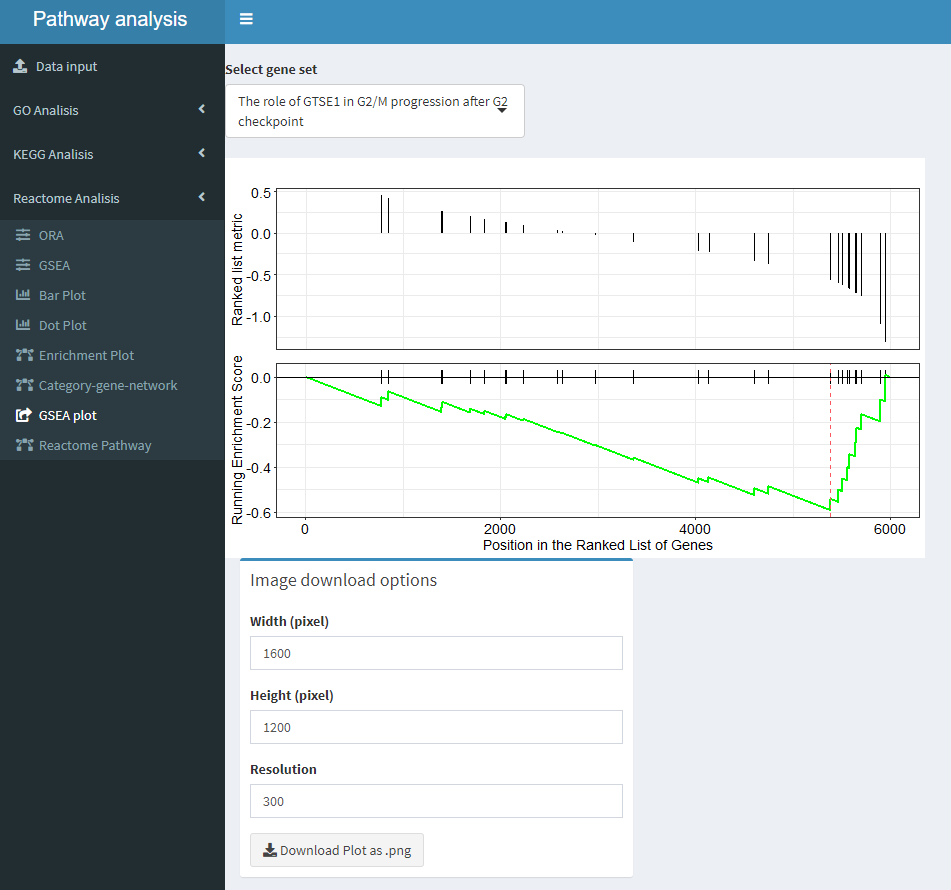
\includegraphics[width=0.6\textwidth]{Estudi1_Fig10_GSEA_RA.png} 
\caption{Gràfic GSEA}
\end{figure}
\end{enumerate}

També podem fer l'anàlisi de KEGG. El resultat de KEGG és similar a l'anàlisi de Reactome. L'aplicació permet però generar les rutes KEGG. Per obtenir-les:

\begin{enumerate}
\item Clico en l'apartat \textit{KEGG Analysis}$\rightarrow$\textit{ORA}. Selecciono com a mètode d'ajustament \textit{BH} i el cut-off del valor de P ajustat 0.05. Clico a \textit{Calculate results}
\begin{figure}[H]
\centering
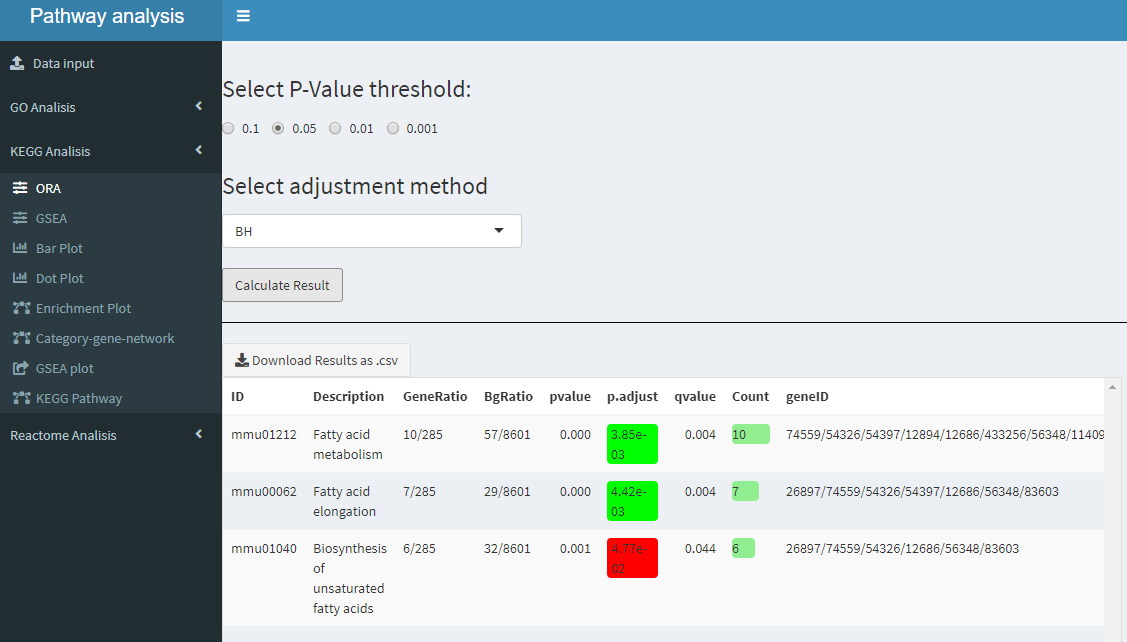
\includegraphics[width=0.6\textwidth]{Estudi1_Fig11_ORA_KEGG.png} 
\caption{Anàlisi ORA de KEGG}
\end{figure}

\item Anem a \textit{KEGG}$\rightarrow$\textit{KEGG Pathway}
\begin{figure}[H]
\centering
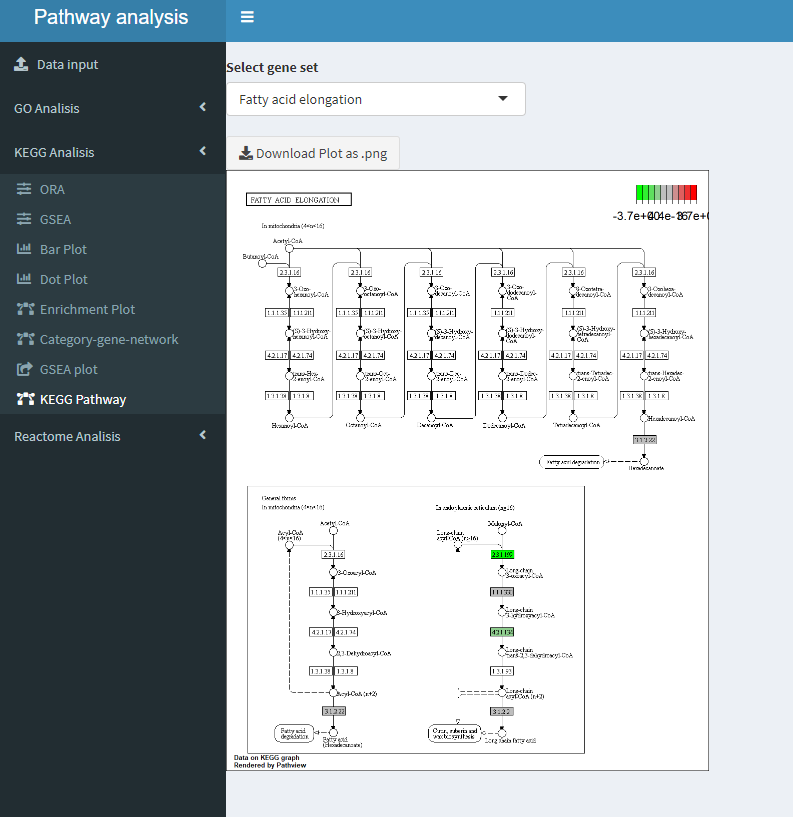
\includegraphics[width=0.6\textwidth]{Estudi1_Fig12_KEGG_Pathway.png} 
\caption{Gràfic de les rutes KEGG}
\end{figure}
\end{enumerate}

L'anàlisi GO no retorna cap terme GO amb el nivell de significació de 0.05. Pujant el nivell de significació fins 0.1 retorna un llistat dels termes enriquits per als components cel·lulars.

Clico en l'apartat \textit{GO Analysis}$\rightarrow$\textit{ORA}. Selecciono com a mètode d'ajustament \textit{BH} i el cut-off del valor de P ajustat 0.1. Selecciono també \textit{CC}. Clico a \textit{Calculate results}
\begin{figure}[H]
\centering
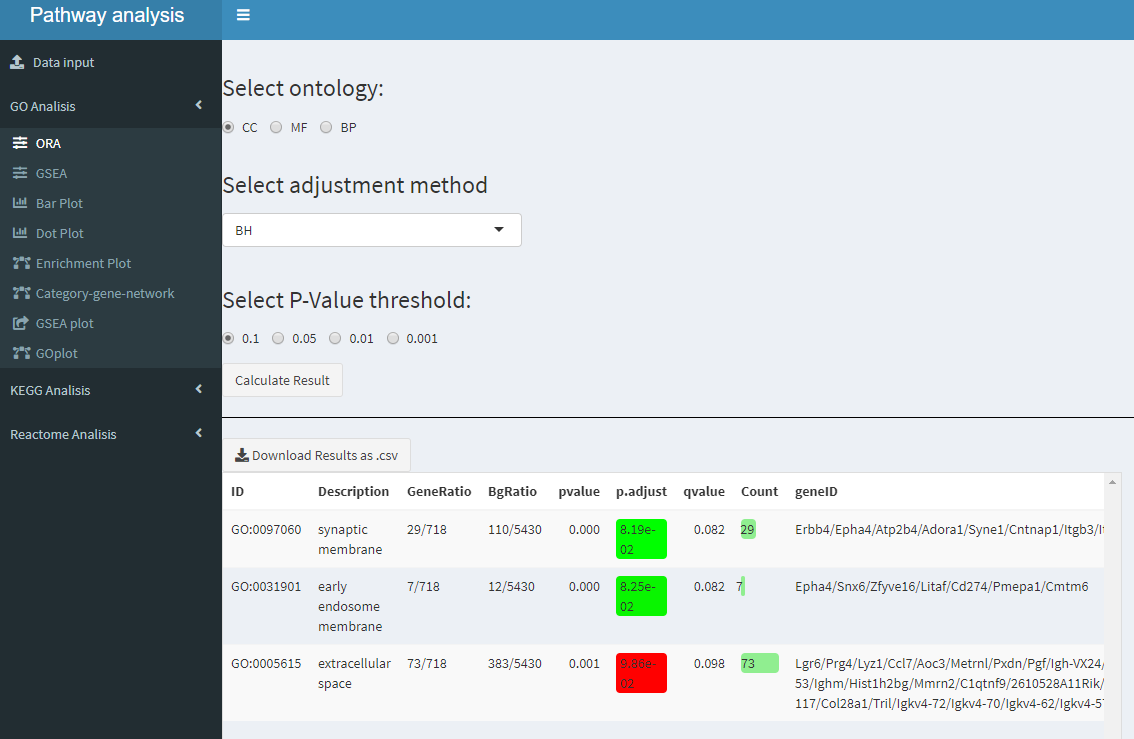
\includegraphics[width=0.6\textwidth]{Estudi1_Fig13_GO.png} 
\caption{L'anàlisi ORA de GO}
\end{figure}


\section{Activitats no previstes}

Treballant en el projecte he notat la necessitat de fer tot el procès més segur. El moment clau era quan no he pogut trobar l'USB on he guardat el meu projecte. Ho tenia en un USB perquè hi treballava ded de molts ordinadors diferents: de casa, de la feina, en un portàtil quan era de viatge. Per tan he decidit guardar tot el projecte en github.com. He creat un repositori al qual puc accedir des d'ordinadors diferents.

\begin{figure}[H]
\centering
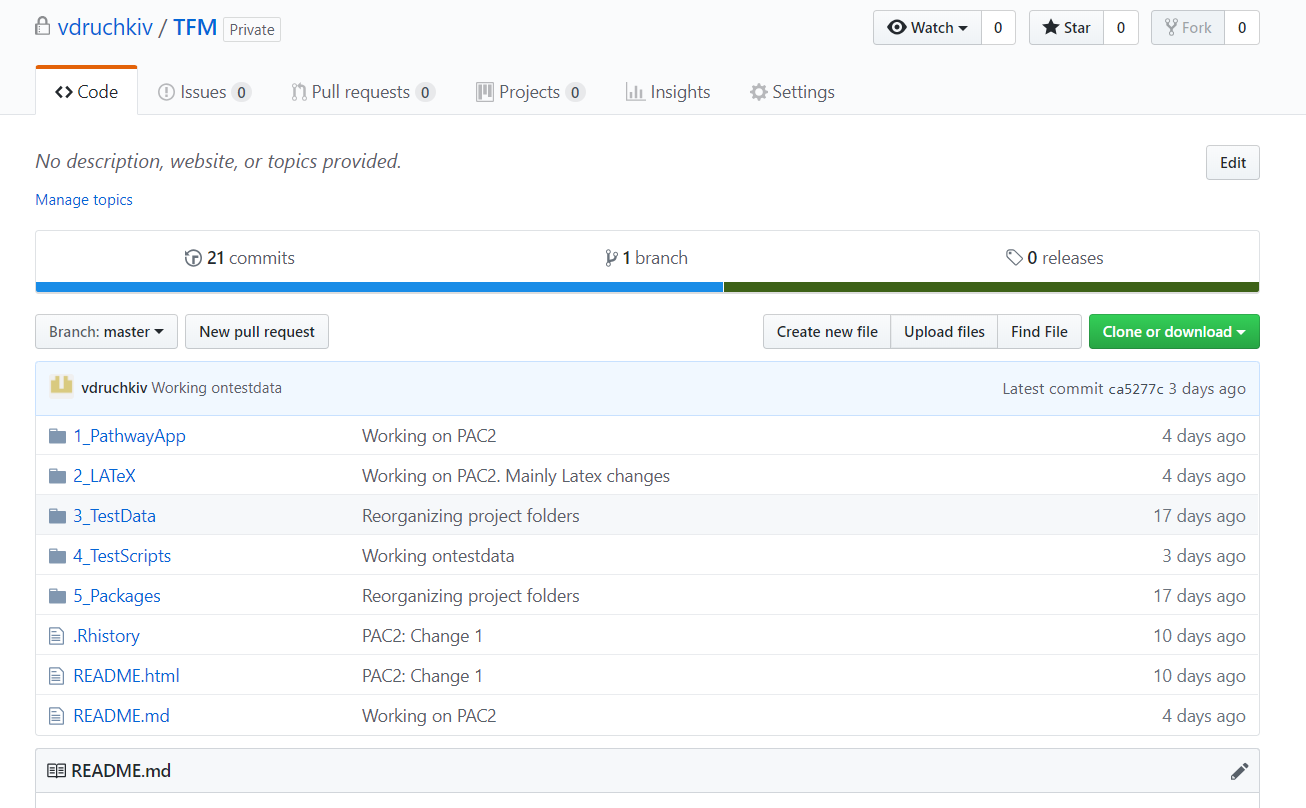
\includegraphics[width=0.9\textwidth]{GitHub.png} 
\caption{Github repositori del TFM}
\end{figure}

Utilitzant el GitBash es pot documentar els canvis (\helvetica{commit}) i pujar (\helvetica{push}) o baixar (\helvetica{pull}) els arxius. Així el treball en el projecte és més segur i pràctic.

\section*{Biblilografia}
\addcontentsline{toc}{section}{Biblilografia}

\begingroup
\renewcommand{\section}[2]{}%
%\renewcommand{\chapter}[2]{}% for other classes
\bibliography{references}
\endgroup
\bibliographystyle{apalike}


\newpage
\section*{Apèndix}
\addcontentsline{toc}{section}{Apèndix}
\appendix 
\section{Els paquets i funcions utilitzats en el app}
\label{sec:A1}
\begingroup\fontsize{8}{10}\selectfont
\begin{longtable}{ll}
\toprule
Package & Funcion\\
\midrule
\rowcolor{gray!6} c("package:clusterProfiler", "package:ReactomePA") & cnetplot\\
c("package:clusterProfiler", "package:ReactomePA") & dotplot\\
\rowcolor{gray!6} c("package:clusterProfiler", "package:ReactomePA") & emapplot\\
c("package:clusterProfiler", "package:ReactomePA") & gseaplot\\
\rowcolor{gray!6} c("package:dplyr", "package:stats") & filter\\
c("package:kableExtra", "package:knitr") & kable\\
\rowcolor{gray!6} c("package:shinydashboard", "package:graphics") & box\\
character(0) & enrichrekegg\\
\rowcolor{gray!6} character(0) & enrichresgo\\
character(0) & enrichresgo\_gsea\\
\rowcolor{gray!6} character(0) & enrichreskegg\\
character(0) & enrichreskegg\_gsea\\
\rowcolor{gray!6} character(0) & enrichresRA\\
character(0) & enrichresRA\_gsea\\
\rowcolor{gray!6} character(0) & geneList\\
character(0) & genes\\
\rowcolor{gray!6} character(0) & kegg\_organism1\\
character(0) & kegg\_organism2\\
\rowcolor{gray!6} character(0) & PathPlotRA\\
character(0) & pathview\\
\rowcolor{gray!6} package:base & abs\\
package:base & as.character\\
\rowcolor{gray!6} package:base & as.numeric\\
package:base & c\\
\rowcolor{gray!6} package:base & file.copy\\
package:base & formatC\\
\rowcolor{gray!6} package:base & length\\
package:base & library\\
\rowcolor{gray!6} package:base & list\\
package:base & max\\
\rowcolor{gray!6} package:base & names\\
package:base & ncol\\
\rowcolor{gray!6} package:base & nrow\\
package:base & paste0\\
\rowcolor{gray!6} package:base & print\\
package:base & return\\
\rowcolor{gray!6} package:base & sort\\
package:base & tempdir\\
\rowcolor{gray!6} package:base & tempfile\\
package:clusterProfiler & enrichGO\\
\rowcolor{gray!6} package:clusterProfiler & enrichKEGG\\
package:clusterProfiler & goplot\\
\rowcolor{gray!6} package:clusterProfiler & gseGO\\
package:clusterProfiler & gseKEGG\\
\rowcolor{gray!6} package:clusterProfiler & search\_kegg\_organism\\
package:dplyr & everything\\
\rowcolor{gray!6} package:dplyr & mutate\\
package:dplyr & select\\
\rowcolor{gray!6} package:formattable & color\_bar\\
package:formattable & color\_tile\\
\rowcolor{gray!6} package:graphics & barplot\\
package:grDevices & dev.off\\
\rowcolor{gray!6} package:grDevices & png\\
package:kableExtra & kable\_styling\\
\rowcolor{gray!6} package:kableExtra & scroll\_box\\
package:png & readPNG\\
\rowcolor{gray!6} package:ReactomePA & enrichPathway\\
package:ReactomePA & gsePathway\\
\rowcolor{gray!6} package:ReactomePA & viewPathway\\
package:shiny & actionButton\\
\rowcolor{gray!6} package:shiny & downloadButton\\
package:shiny & downloadHandler\\
\rowcolor{gray!6} package:shiny & eventReactive\\
package:shiny & fileInput\\
\rowcolor{gray!6} package:shiny & fluidRow\\
package:shiny & h3\\
\rowcolor{gray!6} package:shiny & hr\\
package:shiny & HTML\\
\rowcolor{gray!6} package:shiny & htmlOutput\\
package:shiny & icon\\
\rowcolor{gray!6} package:shiny & imageOutput\\
package:shiny & numericInput\\
\rowcolor{gray!6} package:shiny & radioButtons\\
package:shiny & reactive\\
\rowcolor{gray!6} package:shiny & renderImage\\
package:shiny & renderText\\
\rowcolor{gray!6} package:shiny & renderUI\\
package:shiny & req\\
\rowcolor{gray!6} package:shiny & selectInput\\
package:shiny & shinyApp\\
\rowcolor{gray!6} package:shiny & sliderInput\\
package:shiny & strong\\
\rowcolor{gray!6} package:shiny & tableOutput\\
package:shiny & textInput\\
\rowcolor{gray!6} package:shiny & textOutput\\
package:shiny & uiOutput\\
\rowcolor{gray!6} package:shinycssloaders & withSpinner\\
package:shinydashboard & dashboardBody\\
\rowcolor{gray!6} package:shinydashboard & dashboardHeader\\
package:shinydashboard & dashboardPage\\
\rowcolor{gray!6} package:shinydashboard & dashboardSidebar\\
package:shinydashboard & menuItem\\
\rowcolor{gray!6} package:shinydashboard & sidebarMenu\\
package:shinydashboard & tabItem\\
\rowcolor{gray!6} package:shinydashboard & tabItems\\
package:utils & head\\
\rowcolor{gray!6} package:utils & read.csv\\
package:utils & write.csv\\
\bottomrule
\end{longtable}
\endgroup{}


\end{document}


